% Options for packages loaded elsewhere
\PassOptionsToPackage{unicode}{hyperref}
\PassOptionsToPackage{hyphens}{url}
%
\documentclass[
  12pt,
]{article}
\usepackage{amsmath,amssymb}
\usepackage{iftex}
\ifPDFTeX
  \usepackage[T1]{fontenc}
  \usepackage[utf8]{inputenc}
  \usepackage{textcomp} % provide euro and other symbols
\else % if luatex or xetex
  \usepackage{unicode-math} % this also loads fontspec
  \defaultfontfeatures{Scale=MatchLowercase}
  \defaultfontfeatures[\rmfamily]{Ligatures=TeX,Scale=1}
\fi
\usepackage{lmodern}
\ifPDFTeX\else
  % xetex/luatex font selection
\fi
% Use upquote if available, for straight quotes in verbatim environments
\IfFileExists{upquote.sty}{\usepackage{upquote}}{}
\IfFileExists{microtype.sty}{% use microtype if available
  \usepackage[]{microtype}
  \UseMicrotypeSet[protrusion]{basicmath} % disable protrusion for tt fonts
}{}
\makeatletter
\@ifundefined{KOMAClassName}{% if non-KOMA class
  \IfFileExists{parskip.sty}{%
    \usepackage{parskip}
  }{% else
    \setlength{\parindent}{0pt}
    \setlength{\parskip}{6pt plus 2pt minus 1pt}}
}{% if KOMA class
  \KOMAoptions{parskip=half}}
\makeatother
\usepackage{xcolor}
\usepackage[margin=1in]{geometry}
\usepackage{graphicx}
\makeatletter
\def\maxwidth{\ifdim\Gin@nat@width>\linewidth\linewidth\else\Gin@nat@width\fi}
\def\maxheight{\ifdim\Gin@nat@height>\textheight\textheight\else\Gin@nat@height\fi}
\makeatother
% Scale images if necessary, so that they will not overflow the page
% margins by default, and it is still possible to overwrite the defaults
% using explicit options in \includegraphics[width, height, ...]{}
\setkeys{Gin}{width=\maxwidth,height=\maxheight,keepaspectratio}
% Set default figure placement to htbp
\makeatletter
\def\fps@figure{htbp}
\makeatother
\setlength{\emergencystretch}{3em} % prevent overfull lines
\providecommand{\tightlist}{%
  \setlength{\itemsep}{0pt}\setlength{\parskip}{0pt}}
\setcounter{secnumdepth}{5}
\usepackage{setspace,lscape} \usepackage{amsmath} \usepackage{caption,subcaption,multirow} \usepackage[hang]{footmisc} \usepackage{enumitem} \usepackage{standalone} \renewcommand{\arraystretch}{1.5} \captionsetup[table]{skip=5pt} \setstretch{1.5} \setlength{\parindent}{1em} \setlength{\footnotemargin}{3mm} \setlength{\footnotesep}{3mm}
\ifLuaTeX
  \usepackage{selnolig}  % disable illegal ligatures
\fi
\usepackage[]{natbib}
\bibliographystyle{apalike}
\IfFileExists{bookmark.sty}{\usepackage{bookmark}}{\usepackage{hyperref}}
\IfFileExists{xurl.sty}{\usepackage{xurl}}{} % add URL line breaks if available
\urlstyle{same}
\hypersetup{
  pdftitle={An Attentional Model of Time Discounting},
  pdfauthor={Zark Zijian Wang},
  hidelinks,
  pdfcreator={LaTeX via pandoc}}

\title{An Attentional Model of Time Discounting}
\author{Zark Zijian Wang}
\date{June 05, 2024}

\begin{document}
\maketitle

\hypertarget{introduction}{%
\section{Introduction}\label{introduction}}

decision maker (DM)

Kullback--Leibler~(KL)~divergence~(also called~relative entropy)

hard attention

information avoidance

endogenous time preferences

optimal expectation

we present an axiomatic characterization of AAD with the optimal
discounting framework

\hypertarget{model-setting}{%
\section{Model Setting}\label{model-setting}}

Assume time is discrete. Let
\(s_{0\rightarrow T}\equiv[s_0,s_1,...,s_T]\) denote a reward sequence
that starts delivering rewards at period 0 and ends at period \(T\). At
each period \(t\) of \(s_{0\rightarrow T}\), a specific reward \(s_t\)
is delivered, where \(t\in\{0,1,…,T\}\). Throughout this paper, we only
consider non-negative rewards and finite length of sequence, i.e.~we set
\(s_t \in \mathbb{R}_{\geq 0}\) and \(1\leq T<\infty\). The DM's choice
set is constituted by a range of alternative reward sequences which
start from period 0 and end at some finite period. When making an
intertemporal choice, the DM seeks to find a reward sequence
\(s_{0\rightarrow T}\) in her choice set, which has the highest value
among all alternative reward sequences. To calculate the value of each
reward sequence, we admit the additive discounted utility framework. The
value of \(s_{0\rightarrow T}\) is defined as
\(U(s_{0\rightarrow T})\equiv \sum_{t=0}^T w_{t}u(s_t)\), where
\(u(s_t)\) is the instantaneous utility of receiving \(s_t\), and
\(w_t\) is the decision weight (sometimes called discount factors)
assigned to \(s_t\). We assume the function
\(u:\mathbb{R}\rightarrow \mathbb{R}\) is strictly increasing and for
any \(s>0\), we have \(u(s)>0\). For convenience, we set \(u(0)=0\).

The determination of \(w_t\) is central to this paper. We believe that,
due to the DM's limited attention and demand for information, the DM
tends to overweight the large rewards and underweight the small rewards
within the sequence. Specifically, we suggest \(w_t\) follow a
(generalized) softmax function. We define any decision weight in this
style as an \emph{attention-adjusted discount} factors (AAD), as in
Definition 1.

\noindent \textbf{Definition 1}: \emph{Let}
\(\mathcal{W}\equiv[w_0,...,w_T]\) \emph{denote the decision weights for
all specific rewards in} \(s_{0\rightarrow T}\)\emph{.} \(\mathcal{W}\)
\emph{is called attention-adjusted discount factors (AADs) if for any}
\(t\in\{0,1,…,T\}\),\[\tag{1}
w_t = \frac{d_te^{u(s_t)/\lambda}}{\sum_{\tau=0}^T d_\tau e^{u(s_\tau)/\lambda}} 
\]\emph{where} \(d_t > 0\)\emph{,} \(\lambda>0\)\emph{,} \(u(.)\)
\emph{is the utility function.}

In intuition, how Definition 1 reflects the role of attention in
valuating reward sequences can be explained with four points. First,
each reward in a sequence could be viewed as an information source and
we assume the DM allocates limited information-processing resources
across those information sources. The AADs capture this notion by
normalizing the discount factors, i.e.~fixing the sum of decision
weights at 1. Similar assumptions are typically used in recursive
preferences, such as \citet{epstein1989substitution} and
\citet{weil1990nonexpected}. In this paper, the implication of
normalization assumption is twofold. First, increasing the decision
weight of one reward would reduce the decision weights of other rewards
in the sequence, implying that focusing on one reward would make DM
insensitive to the values of other rewards. Second, when there are more
rewards in the sequence, DM needs to split attention across a wider
range to process each of them, which may reduce the attention to, or
decision weight of, each individual reward.

Second, \(w_t\) is strictly increasing with \(s_t\), indicating that DM
would pay more attention to larger rewards. This is consistent with many
empirical studies that suggest people tend to pay more attention to
information associated with larger rewards. For instance, people perform
a ``value-driven attentional capture'' effect in visual search
\citep{della2009learning, hickey2010reward, anderson2011value, chelazzi2013rewards, jahfari2017sensitivity}.
In one study \citep{anderson2011value}, researchers recruit participants
to do a series of visual search tasks, in each of which participants can
earn a reward after detecting a target object from distractors. If an
object is set as the target and is associated with a large reward, it
can capture more attention even for the succeeding tasks. Therefore, in
one following task, presenting this object as a distractor will slow
down target detection.\footnote{Some scholars may classify attention
  into two categories: ``bottom-up control'' and ``top-down control''.
  However, the evidence about value-driven attentional capture does not
  fall into either of these categories. Thus, in this paper, we do not
  describe attention with this dichotomy. Instead, we view attention as
  a mechanism that seeks to maximize the utility of information.} In
addition, in financial decision making, investors usually perform an
ostrich effect \citep{galai2006ostrich, karlsson2009ostrich}. One
relevant evidence is that stock traders log in their brokerage accounts
less frequently after market declines \citep{sicherman2016financial}.

Third, \(w_t\) is ``anchored'' in a reference weight \(d_t\). For a
certain sequence of rewards, \(d_t\) could denote the initial weight
that the DM would assign to a reward delivered at period \(t\) without
knowing its realization. The determination of \(d_t\) is mediated by the
difficulty to mentally represent a future event
\citep{trope2003temporal} and the frequency of time delays in a global
context \citep{stewart2006decision}. The constraint on the deviation
between \(w_t\) and \(d_t\) indicates that reallocating attention or
acquiring new information is costly. The deviation of \(w_t\) from
\(d_t\) depends on parameter \(\lambda\), which as we discuss in the
next section, can reflect the unit cost of attention adjustment. A large
\(\lambda\) implies a low learning rate and a high cognitive cost in
adapting the decision weights to the local context.

Fourth, we adopt the idea of \citet{gottlieb2012attention} and
\citet{gottlieb2013information} that attention can be understood as an
active information-sampling mechanism which selects information based on
the perceived utility of information. For intertemporal choices, we
assume the DM would selectively sample value information from each
reward (information source) when processing a reward sequence, and the
AAD can represent an approximately optimal sampling strategy. Note that
the AADs follow a softmax function. \citet{matvejka2015rational} and
\citet{mackowiak2023rational} claim that if a behavioral strategy
conforms to this type of function, then it can be interpreted as a
solution to some optimization problem under information constraints.

\hypertarget{interpretation}{%
\section{Interpretation}\label{interpretation}}

\hypertarget{information-maximizing-exploration}{%
\subsection{\texorpdfstring{Information Maximizing Exploration
\label{info_exploration}}{Information Maximizing Exploration }}\label{information-maximizing-exploration}}

In this section, we provide two approaches to characterize AAD: the
first is based on information maximizing exploration, and the second is
based on optimal discounting. These approaches are closely related to
the idea proposed by \citet{gottlieb2012attention},
\citet{gottlieb2013information} and \citet{sharot2020people}, that
people tend to pay attention to information with high \emph{instrumental
utility} (help identifying the optimal action), \emph{cognitive utility}
(satisfying curiosity), or \emph{hedonic utility} (inducing positive
feelings). It is worth mentioning that the well-known rational
inattention theories are grounded in the instrumental utility of
information.\footnote{The rational inattention theory assumes the DM
  learns information about different options in order to find the best
  option. For details, see \citet{sims2003implications},
  \citet{matvejka2015rational}, and \citet{mackowiak2023rational}.}
Instead, in this paper, we draw on the cognitive and hedonic utility of
information to build our theory of time discounting. Our first approach
to characterizing AAD is relevant to the cognitive utility: the DM's
information acquisition process is curiosity-driven. The model setting
of this approach, similar with \citet{gottlieb2012attention} and
\citet{gottlieb2013information}, is based on a reinforcement learning
framework. Specifically, we assume the DM seeks to maximize the
information gain with a commonly-used exploration strategy. Our second
approach is relevant to the hedonic utility: the DM consider the
feelings of multiple selves and seeks to maximize their total utility
under some cognitive cost. The theoretical background for the second
approach is \citet{noor2022optimal,noor2024constrained}. We describe the
first approach in this subsection and the second approach in Section
\ref{optimal_discount}.

For the information maximizing exploration approach, we assume that
before having any information of a reward sequence, the DM perceives it
has no value. Then, each reward in the sequence \(s_{0\rightarrow T}\)
is processed as an individual information source. The DM engages her
attention to actively sample signals at each information source and
update her belief about the sequence value accordingly. The signals are
noisy. For any \(t\in\{0,1,…,T\}\), the signal sampled at information
source \(s_t\) could be represented by \(x_t =u(s_t)+\epsilon_t\), where
each \(\epsilon_t\) is i.i.d. and
\(\epsilon_t \sim N(0,\sigma_\epsilon^2)\). The sampling weight for
information source \(s_t\) is denoted by \(w_t\).

The DM's belief about the sequence value \(U(s_{0\rightarrow T})\) is
updated as follows. At first, she holds a prior \(U_0\), and given she
perceives no value from the reward sequence, the prior could be
represented by \(U_0 \sim N(0, \sigma^2)\). Second, she draws a series
of signals at each information source \(s_t\). Note we define
\(U(s_{0\rightarrow T})\) as a weighted mean of instantaneous utilities,
i.e.~\(U(s_{0\rightarrow T})=\sum_{t=0}^Tw_tu(s_t)\). Let \(\bar{x}\)
denote the mean sample signal and \(U\) denote a realization of
\(U(s_{0\rightarrow T})\). If there are \(k\) signals being sampled in
total, we should have
\(\bar{x} | U, \sigma_\epsilon\sim N(U,\frac{\sigma_{\epsilon}^2}{k})\).
Third, she uses the sampled signals to infer \(U(s_{0\rightarrow T})\)
in a Bayesian fashion. Let \(U_k\) denote the valuer's posterior about
the sequence value after receiving \(k\) signals. According to the
Bayes' rule, we have \(U_k\sim N(\mu_k,\sigma_k^2)\) and\[
\mu_k = \frac{k^2\sigma_\epsilon^{-2}}{\sigma^{-2}+k^2\sigma_\epsilon^{-2}}\bar{x}\qquad,\qquad 
\sigma_k^2 =  \frac{1}{\sigma^{-2}+k^2\sigma_\epsilon^{-2}}
\]We assume the DM takes \(\mu_k\) as the valuation of reward sequence.
It is clear that as \(k\rightarrow \infty\), the sequence value will
converge to the mean sample signal, i.e.~\(\mu_k \rightarrow \bar{x}\).

The DM's goal of sampling signals is to maximize her information gain.
The information gain is defined as the KL divergence from the prior
\(U_0\) to the posterior \(U_k\). In intuition, the KL divergence
provides a measure for distance between distributions. As the DM
acquires more information about \(s_{0\rightarrow T}\), her posterior
belief should move farther away from the prior. We let \(p_0(U)\) and
\(p_k(U)\) denote the probability density functions of \(U_0\) and
\(U_k\). Then, the information gain is\[\tag{2}
\begin{aligned}
D_{KL}(U_k||U_0)&=\int_{-\infty}^{\infty} p_k(U) \log\left(p_k(U)/p_0(U)\right)dU \\
&=\frac{\sigma_k^2+\mu_k^2}{2\sigma^2} - \log\left(\frac{\sigma_k}{\sigma}\right)-\frac{1}{2}
\end{aligned}
\]Notably, in Equation (2), \(\sigma_k\) depends only on sample size
\(k\) and \(\mu_k\) is proportional to \(\bar{x}\). Therefore, the
problem of maximizing \(D_{KL}(U_k||U_0)\) could be reduced to
maximizing \(\bar{x}\) (as each \(u(s_t)\) is non-negative). The reason
is that, drawing more samples can always increase the precision of the
DM's estimate about \(U(s_{0\rightarrow T})\), and a larger \(\bar{x}\)
implies more ``surprises'' in comparison to the DM's initial perception
that \(s_{0\rightarrow T}\) contains no value.

Maximizing the mean sample signal \(\bar{x}\) under a limited sample
size \(k\) is actually a multi-armed bandit problem
\citep[][Ch.2]{sutton2018reinforcement}. On the one hand, the DM wants
to draw more samples at information sources that are known to produce
greater value signals (exploit). On the other hand, she wants to learn
some value information from other information sources (explore). We
assume the DM would take a softmax exploration strategy to solve this
problem. That is,\[
w_t \propto d_t e^{\bar{x}_t/\lambda}
\]where \(\bar{x}_t\) is the mean sample signal generated by information
source \(s_t\) so far, \(1/\lambda\) is the learning rate, and \(d_t\)
is the initial sampling weight for \(s_t\).\footnote{Classic softmax
  strategy assumes the initial probability of taking an action follows
  an uniform distribution. We relax this assumption by importing
  \(d_t\), so that the DM can hold an initial preference of sampling
  over the dated rewards.} Note \(\bar{x_t}\) cannot be calculated
without doing simulations under a certain \(\sigma_\epsilon\). For
researchers, modelling an intertemporal choice in this way requires
conducting a series of simulations and then calibrating
\(\sigma_\epsilon\) for every choiceable option, which could be
computationally expensive. Fortunately, according to the weak law of
large numbers, as the sample size \(k\) gets larger, \(\bar{x}_t\) is
more likely to fall into a neighborhood of \(u(s_t)\). Thus, the AAD
which assumes \(w_t \propto d_t e^{u(s_t)/\lambda}\) could be viewed as
a proper approximation to the softmax exploration strategy.

Those who familiar with reinforcement learning algorithms may notice
that here \(u(s_t)\) is a special case of action-value function
(assuming the learner only cares about the value of current reward in
her each draw of the sample). The AAD thus can be viewed as a specific
version of the soft Q-learning or policy gradient method for solving the
given multi-armed bandit problem
\citep{haarnoja2017reinforcement, schulman2017equivalence}. Such methods
are widely used (and sample-efficient) in reinforcement learning.
Moreover, one may argue that the applicability of softmax exploration
strategy is subject to our model assumptions. Under alternative
assumptions, the strategy may not be ideal. We acknowledge this
limitation and suggest that researchers interested in modifying our
model consider different objective functions or different families of
noises. For example, if the DM aims to minimize the regret rather than
maximizing \(\bar{x}\), the softmax exploration strategy can produce
suboptimal actions and one remedy is to use the Gumbel--softmax strategy
\citep{cesa2017boltzmann}. If noises \(\epsilon_0,...,\epsilon_T\) do
not follow an i.i.d normal distribution, the information gain
\(D_{KL}(U_k||U_0)\) may be complex to compute, thus one can use its
variational bound as the objective \citep{houthooft2016vime}. Compared
to these complex settings, the model setting in this subsection aims to
provides a simple benchmark for understanding the role of attention in
mental valuation of a reward sequence.

Two strands of literature can help justify the assumptions we use in
information maximizing exploration approach. First, models based on the
assumption that DM seeks to maximize the information gain between the
posterior and prior beliefs has been studied extensively both in
cognitive psychology
\citep{oaksford1994rational, itti2009bayesian, friston2017active} and
machine learning literature \citep{settles2009active, ren2021survey}. In
one study, \citet{itti2009bayesian} find this assumption has a strong
predictive power for visual attention. Our assumption that the DM
updates decision weights toward a greater \(D_{KL}(U_k||U_0)\) is
generally consistent with this finding. Second, the softmax exploration
strategy is widely used by neuroscientists in studying human
reinforcement learning
\citep{daw2006cortical, fitzgerald2012action, collins2014opponent, niv2015reinforcement, leong2017dynamic}.
For instance, \citet{daw2006cortical} find the softmax strategy can
characterize humans' exploration behavior better than other classic
strategies (e.g. \(\epsilon\)-greedy). \citet{collins2014opponent} show
that models based on the softmax strategy exhibit a good performance in
explaining the striatal dopaminergic system's activities (which is
central in brain's sensation of pleasure and learning of rewarding
actions) in reinforcement learning tasks.

\hypertarget{optimal-discounting}{%
\subsection{\texorpdfstring{Optimal Discounting
\label{optimal_discount}}{Optimal Discounting }}\label{optimal-discounting}}

The second approach to characterize AAD is based on the optimal
discounting model \citep{noor2022optimal,noor2024constrained}. In one
version of this model, the authors assume that the DM has a limited
capacity of attention (or in their term, ``empathy''), and before
evaluating a reward sequence \(s_{0\rightarrow T}\), she naturally
focuses on the current period. The instantaneous utility \(u(s_t)\)
represents the well-being that the DM's self of period \(t\) can obtain
from the reward sequence. For valuating \(s_{0\rightarrow T}\), the DM
needs to split attention over \(T\) time periods to consider the feeling
of each self. This re-allocation of attention is cognitive costly. The
DM seeks to find a balance between improving the overall well-being of
multiple selves and reducing the incurred cognitive cost.
\citet{noor2022optimal,noor2024constrained} specify an optimization
problem to capture this decision. In this paper, we adopt a variant of
their original model. The formal definition of the optimal discounting
problem is given by Definition 2. \footnote{There are three differences
  between Definition 2 and the original optimal discounting model
  \citep{noor2022optimal,noor2024constrained}. First, in our setting,
  shifting attention to future rewards may reduce the attention to the
  current reward, while this would never happen in
  \citet{noor2022optimal,noor2024constrained}. Second, the original
  model assumes \(f'_t(w_t)\) must be continuous at 0 and \(w_t\) must
  be no larger than 1. We relax these assumptions since neither
  \(w_t=0\) nor \(w_t\geq1\) is included our solutions. Third, the
  original model assumes that \(f'_t(w_t)\) is left-continuous in
  \([0,1]\), and there exist \(\underline{w},\bar{w}\in[0,1]\) such that
  \(f'_t(w_t)=0\) when \(w_t\leq\underline{w}\), \(f'_t(w_t)=\infty\)
  when \(w_t\geq\bar{w}\), and \(f'_t(w_t)\) is strictly increasing when
  \(w_t \in [\underline{w},\bar{w}]\). We simplify this assumption by
  setting \(f'_t(w_t)\) is continuous strictly increasing in \((0,1)\).
  For how \(f'_t(w_t)\) would behave near the border of \([0,1]\), we
  set \(\lim_{w_t\rightarrow 0} f'_t(w_t)=-\infty\) instead.}

\noindent \textbf{Definition 2}: \emph{Given reward sequence}
\(s_{0\rightarrow T}=[s_0,...,s_T]\)\emph{, the following optimization
problem is called an optimal discounting problem for}
\(s_{0\rightarrow T}\)\emph{:}\[
\begin{aligned}
&\max_{\mathcal{W}}\;&&\sum_{t=0}^T w_tu(s_t) - C(\mathcal{W}) \\
&s.t.\; &&\sum_{t=0}^Tw_t \leq M \\
&&& w_t \geq 0 \text{ for all } t\in \{0,1,...,T\}
\end{aligned}
\]\emph{where} \(M>0\)\emph{,} \(C(\mathcal{W})\geq 0\). For any
\(t\in\{0,1,…,T\}\), \(u(s_t)<\infty\). \(C(\mathcal{W})\) \emph{is the
cognitive cost function and is constituted by time-separable costs,
i.e.} \(C(\mathcal{W})=\sum_{t=0}^Tf_t(w_t)\)\emph{, where for all}
\(w_t\in(0,1)\)\emph{,} \(f_t(w_t)\) \emph{is differentiable.}
\(f'_t(w_t)\) \emph{is continuous and} stric\emph{tly increasing, and}
\(\lim_{w_t\rightarrow 0} f'_t(w_t)=-\infty\).

Here \(w_t\) reflects the attention paid to consider the feeling of
\(t\)-period self. The DM's objective function is the attention-weighted
sum of utilities obtained by the multiple selves minus the cognitive
cost of attention re-allocation. As is illustrated by
\citet{noor2022optimal,noor2024constrained}, a key feature of this model
is that decision weight \(w_t\) is increasing with \(s_t\), indicating
the DM tends to pay more attention to larger rewards. Moreover, it is
easy to validate that if the following three conditions are satisfied,
the solution to the optimal discounting problem will take an AAD form:

\begin{enumerate}
\def\labelenumi{(\roman{enumi})}
\item
  The constraint on sum of decision weights is always tight. That is,
  \(\sum_{t=0}^Tw_t=M\). Without loss of generality, we can set \(M=1\).
\item
  There exists a realization of decision weights
  \(\mathcal{D}=[d_0,...,d_T]\) such that \(d_t>0\) for all
  \(t\in\{0,…,T\}\) and the cognitive cost is proportional to the KL
  divergence from \(\mathcal{D}\) to the DM's strategy \(\mathcal{W}\)
  where applicable. That is,
  \(C(\mathcal{W})= \lambda\cdot D_{KL}(\mathcal{W}||\mathcal{D})\),
  where \(\lambda>0\).
\end{enumerate}

Here \(d_t\) sets a reference for determining the decision weight
\(w_t\), the parameter \(\lambda\) indicates how costly the attention
re-allocation process is, and
\(D_{KL}(\mathcal{W}||\mathcal{D})=\sum_{t=0}^Tw_t\log(\frac{w_t}{d_t})\).
The solution to the optimal discounting problem under condition (i)-(ii)
can be derived in the same way as Theorem 1 in
\citet{matvejka2015rational}. Note this solution is equivalent to that
of a bounded rationality model: assuming the DM wants to find a
\(\mathcal{W}\) that maximizes \(\sum_{t=0}^Tw_tu(s_t)\) but can only
search for solutions within a KL neighborhood of \(\mathcal{D}\).
Related models can also be found in \citet{todorov2009efficient}.

We interpret the implications of condition (i)-(ii) with behavioral
axioms. Note if each \(s_t\) is an independent option and
\(\mathcal{W}\) simply represents the DM's choice strategy across
options, then these condition can be characterized by rational
inattention theories, e.g. \citet{caplin2022rationally}. However, here
\(\mathcal{W}\) is a component of sequence value
\(U(s_{0\rightarrow T})\), and the DM is assumed to choose the option
with highest sequence value. Thus, the behavioral implications of
condition (i)-(ii) should be derived in different ways\emph{.} To
illustrate, let \(\succsim\) denote the preference relation between two
reward sequences.\footnote{If \(a \succsim b\) and \(b\succsim a\), we
  say \(a\sim b\) (``\(a\) is the same good as \(b\)''). If
  \(a \succsim b\) does not hold, we say \(b\succ a\) (``\(b\) is better
  than \(a\)''). \(\succsim\) can also characterize the preference
  relation between single rewards as the single rewards can be viewed as
  one-period sequences.} For any reward sequence
\(s_{0\rightarrow T}=[s_0,...,s_T]\), we define
\(s_{0\rightarrow t}=[s_0,...,s_t]\) as a sub-sequence of it, where
\(1\leq t\leq T\).\footnote{Notably, every sub-sequence starts with
  period 0.} We first introduce two axioms for \(\succsim\):

\noindent \textbf{Axiom 1}: \(\succsim\) \emph{has the following
properties:}

\begin{enumerate}
\def\labelenumi{(\alph{enumi})}
\item
  \emph{(complete order)} \(\succsim\) \emph{is complete and
  transitive.}
\item
  \emph{(continuity) For any reward sequences} \(s,s'\) \emph{and
  reward} \(c\in \mathbb{R}_{\geq 0}\)\emph{, the sets}
  \(\{\alpha \in(0,1) | \alpha\cdot s + (1-\alpha)\cdot c \succsim s'\}\)
  \emph{and}
  \(\{\alpha \in(0,1) | s' \succsim \alpha\cdot s + (1-\alpha)\cdot c \}\)
  \emph{are closed.}
\item
  \emph{(state-independent) For any reward sequences} \(s,s'\) \emph{and
  reward} \(c\in \mathbb{R}_{\geq 0}\)\emph{,} \(s \succsim s'\)
  \emph{implies for any} \(\alpha \in (0,1)\)\emph{,}
  \(\alpha\cdot s + (1-\alpha)\cdot c \sim \alpha \cdot s' + (1-\alpha) \cdot c\)\emph{.}
\item
  \emph{(reduction of compound alternatives) For any reward sequences}
  \(s,s',y\) \emph{and rewards}
  \(c_1,c_2\in \mathbb{R}_{\geq 0}\)\emph{, if there exist}
  \(\alpha, \beta \in (0,1)\) \emph{such that}
  \(s \sim \alpha \cdot y + (1-\alpha) \cdot c_1\)\emph{, then}
  \(s' \sim \beta \cdot s + (1-\beta)\cdot c_2\) \emph{implies}
  \(s' \sim \beta\alpha\cdot y+\beta(1-\alpha)\cdot c_1 + (1-\beta)\cdot c_2\)\emph{.}
\end{enumerate}

\noindent \textbf{Axiom 2}: \emph{For any} \(s_{0\rightarrow T}\)
\emph{and any} \(\alpha_1,\alpha_2 \in (0,1)\)\emph{, there exists}
\(c\in \mathbb{R}_{\geq 0}\) \emph{such that}
\(\alpha_1 \cdot s_{0\rightarrow T-1}+\alpha_2\cdot s_T \sim c\)\emph{.}

The two axioms are almost standard in decision theories. The assumption
of complete order implies preferences between reward sequences can be
characterized by an utility function. Continuity and state-independence
ensure that in a stochastic setting where the DM can receive one reward
sequence under some states and receive a single reward under other
states, her preference can be characterized by expected utility
\citep{herstein1953axiomatic}. Reduction of compound alternatives
ensures that the DM's valuation on a reward sequence is constant across
states. Axiom 2 is an extension of the Constant-Equivalence assumption
in \citet{bleichrodt2008koopmans}. It implies there always exists a
constant that can represent the value of a linear combination of
sub-sequence \(s_{0\rightarrow T}\) and the end-period reward \(s_T\),
as long as the weights lie in \((0,1)\).

For a given \(s_{0\rightarrow T}\), the optimal discounting model can
generate a sequence of decision weights \([w_0,...,w_T]\). Furthermore,
the model assumes the DM's preference for \(s_{0\rightarrow T}\) can be
characterized by the preference for
\(w_0\cdot s_0+w_1\cdot s_1 +...+w_T\cdot s_T\). We use Definition 3 to
capture this assumption.\footnote{\citet{noor2022optimal} refer the term
  ``optimal discounting representation'' as Costly Empathy
  representation.}

\noindent \textbf{Definition 3}: \emph{Given reward sequence}
\(s_{0\rightarrow T}=[s_0,...,s_T]\) \emph{and}
\(s'_{0\rightarrow T'}=[s'_0,...,s'_{T'}]\)\emph{, the preference
relation} \(\succsim\) \emph{has an optimal discounting representation
if} \[
s_{0\rightarrow T} \succsim s'_{0\rightarrow T'}\quad
\Longleftrightarrow \quad \sum_{t=0}^T w_t\cdot s_t
\succsim \sum_{t=0}^{T'} w'_t \cdot s'_t
\] \emph{where} \(\{w_t\}_{t=0}^T\) \emph{and} \(\{w'_t\}^{T'}_{t=0}\)
\emph{are solutions to the optimal discounting problems for}
\(s_{0\rightarrow T}\) \emph{and} \(s'_{0\rightarrow T'}\)
\emph{respectively.}

Furthermore, if Definition 3 is satisfied and \(\{w_t\}_{t=0}^T\) as
well as \(\{w'_t\}^{T'}_{t=0}\) takes the AAD form, we say \(\succsim\)
has an \emph{AAD representation}. Now we specify two behavioral axioms
that are key to characterize the AAD functions.

\noindent \textbf{Axiom 3} (sequential outcome-betweenness): \emph{For
any} \(s_{0\rightarrow T}\)\emph{, there exists} \(\alpha\in(0,1)\)
\emph{such that}
\(s_{0\rightarrow T} \sim \alpha\cdot s_{0\rightarrow T-1}+(1-\alpha) \cdot s_T\)\emph{.}

\noindent \textbf{Axiom 4} (sequential bracket-independence):
\emph{Suppose} \(T\geq 2\). \emph{For any} \(s_{0\rightarrow T}\)\emph{,
if there exist} \(\alpha_1,\alpha_2,\beta_0,\beta_1,\beta_2\in(0,1)\)
\emph{such that}
\(s_{0\rightarrow T}\sim \alpha_1 \cdot s_{0\rightarrow T-1} + \alpha_2 \cdot s_{T}\)
\emph{and}
\(s_{0\rightarrow T}\sim \beta_0 \cdot s_{0\rightarrow T-2}+\beta_1 \cdot s_{T-1}+\beta_2 \cdot s_{T}\)\emph{,
then we must have} \(\alpha_2 = \beta_2\)\emph{.}

Axiom 3 implies that for a reward sequence \(s_{0\rightarrow T-1}\), if
we add a new reward \(s_T\) at the end of the sequence, then the value
of the new sequence should lie between the original sequence
\(s_{0\rightarrow T-1}\) and the newly added reward \(s_T\). Notably,
Axiom 3 is consistent with the empirical evidence about \emph{violation
of dominance} \citep{scholten2014better, jiang2017better} in
intertemporal choice. Suppose the DM is indifferent between a
small-sooner reward (SS) ``receive £75 today'' and a large-later reward
(LL) ``receive £100 in 52 weeks''. \citet{scholten2014better} find when
we add a tiny reward after the payment in SS, e.g.~changing SS to
``receive £75 today and £3 in 52 weeks'', the DM would be more likely to
prefer LL over SS. \citet{jiang2017better} find the same effect can
apply to LL. That is, if we add a tiny reward after the payment in LL,
e.g.~changing LL to ``receive £100 in 52 weeks and £3 in 53 weeks'', the
DM may be more likely to prefer SS over LL.

Axiom 4 implies that no matter how the DM brackets the rewards into
sub-sequences (or how the sub-sequences get further decomposed), the
decision weights for rewards outside them should not be affected.
Specifically, suppose we decompose reward sequence
\(s_{0\rightarrow T}\) and find its value is equivalent to a linear
combination of \(s_{0\rightarrow T-1}\) and \(s_T\). We also can further
decompose \(s_{0\rightarrow T-1}\) to a linear combination of
\(s_{0\rightarrow T-2}\) and \(s_{T-1}\). But no matter how we operate,
as long as the decomposition is carried out inside
\(s_{0\rightarrow T-1}\), the weight of \(s_T\) in the valuation of
\(s_{0\rightarrow T}\) will always remain the same. This axiom is an
analog to independence of irrelevant alternatives in discrete choice
problems, while the latter is a key feature of softmax choice function.

We show in Proposition 1 that the optimal discounting model plus Axiom
1-4 can exactly produce AAD.

\noindent \textbf{Proposition 1}: \emph{Suppose} \(\succsim\) \emph{has
an optimal discounting representation, then it satisfies Axiom 1-4 if
and only if has an AAD representation.}

The necessity (``only if'') is easy to see. We present the proof of
sufficiency (``if'') in Appendix A. The sketch of the proof is as
follows. First, by recursively applying Axiom 3 and Axiom 1 to each
sub-sequence of \(s_{0\rightarrow T}\), we can obtain that there is a
sequence of decision weights \(\{w_t\}_{t=0}^T\) such that
\(s_{0\rightarrow T}\sim w_0\cdot s_0+...+w_T\cdot s_T\), and
\(\sum_{t=0}^T w_t = 1\), \(w_t>0\). Second, by the FOC of the optimal
discounting problem, we have \(f'_t(w_t)=u(s_t)+\theta\), where
\(\theta\) is the Lagrangian multiplier. Given \(f'_t(.)\) is continuous
and strictly increasing, we can define its inverse function as
\(\phi_t(.)\) and set \(w_t=\phi_t(u(s_t)+\theta)\). Third, Axiom 4
indicates that the decision weights for rewards outside a reward
sub-sequence is irrelevant to the decision weights in it. Imagine that
we add a new reward \(s_{T+1}\) to the end of \(s_{0\rightarrow T}\) and
denote the decision weights for \(s_{0\rightarrow T+1}\) by
\(\{w'_t\}_{t=0}^{T+1}\). The relative difference between \(w'_t\) and
\(w'_{t-1}\) should be the same as that between \(w_t\) and \(w_{t-1}\)
for all \(1\leq t\leq T\) (similar with the independence of irrelevant
alternative principle). Then, by applying Axiom 4 jointly with Axiom
1-3, we can show \(w_0/w'_0=w_1/w'_1=...=w_T/w'_T\) . Suppose
\(w'_t=\phi_t(u(s_t)-\eta)\), we can obtain
\(w_t \propto e^{\ln\phi_t(u(s_t)-\eta)}\). Fourth, we can adjust
\(s_{T+1}\) arbitrarily to get different realizations of \(\eta\).
Suppose under some \(s_{T+1}\), we have \(w'_t = \phi_t(u(s_t))\), which
indicates \(w_t \propto e^{\ln\phi_t(u(s_t))}\). By combining this with
the proportional relation obtained in the last step, we can conclude
that for some \(\kappa>0\), there must be
\(\ln\phi_t(u(s_t))=\ln\phi_t(u(s_t)-\eta)+\kappa\eta\). This indicates
\(\ln \phi_t(.)\) is linear in a given range of \(\eta\). Finally, we
show that the linear condition holds when
\(\eta\in[0,u_{\max}-u_{\min}]\), where \(u_{\max},u_{\min}\) are the
maximum and minimum instantaneous utilities in \(s_{0\rightarrow T}\).
Therefore, we can rewrite \(\ln\phi_t(u(s_t))\) as
\(\ln\phi_t(u_{\min})+\kappa(u(s_t)-u_{\min})\). Setting
\(d_t=\phi_t(u_{\min})\), \(\lambda =1/\kappa\), and reframing the
utility function, we obtain \(w_t \propto d_t e^{u(s_t)/\lambda}\),
which is AAD.

\hypertarget{implications-for-decision-making}{%
\section{Implications for Decision
Making}\label{implications-for-decision-making}}

\hypertarget{hidden-zero-effect}{%
\subsection{Hidden Zero Effect}\label{hidden-zero-effect}}

Empirical evidence suggests the subjective discount factor of a reward
is dependent not just on delay but also on the framing of reward
sequences. In this subsection, we discuss the evidence of (asymmetric)
hidden zero effect
\citep{magen2008hidden, radu2011mechanism, read2017value}. Similar with
violation of dominance, this effect also provides a justification for
our assumption that the sum of AADs is a fixed amount.

To illustrate, suppose the DM is indifferent between ``receive £100
today'' (SS) and ``receive £120 in 25 weeks'' (LL). The hidden zero
effect suggests that people are more likely to choose LL when SS is
framed as a sequence rather than as a single-period reward. In other
words, if we frame SS as ``receive £100 today and £0 in 25 weeks''
(SS1), the DM would prefer LL to SS1. Moreover, \citet{read2017value}
find that framing LL as ``receive £0 today and £120 in 25 weeks'' (LL1)
has no effect on preference.

The hidden zero effect can be explain by the AAD model. When a DM
valuates a reward sequence \(s_{0\rightarrow T}\), the AAD model assumes
that she splits a fixed amount of attention over \(T\) periods. For the
given example, the DM may perceive the time length of SS as ``today''
and perceives the time length of SS1 as ``25 weeks''. In the former
case, she can focus her attention on the current period when she can get
£100. While in the latter case, she have to spend some attention to
future periods in which no reward is delivered, which also decreases the
decision weight assigned to the current period. As a result, she values
SS1 lower than SS. By contrast, the DM may perceive the time length of
both LL and LL1 as ``25 weeks''. When she valuate LL, she has already
paid some attention to periods earlier than ``25 weeks''. Therefore,
changing LL to LL1 does not change the choice.

\hypertarget{relation-to-hyperbolic-discounting}{%
\subsection{Relation to Hyperbolic
Discounting}\label{relation-to-hyperbolic-discounting}}

Most of the intertemporal choice studies only involve comparisons
between single-period rewards (SS and LL). Here we derive the discount
factor for SS/LL under the AAD model and use that to illustrate how
attention allocation can account for the anomalies in such decision
settings. For simplicity, we assume the reference weight
\(d_t = \delta^t\), \(\delta\in(0,1]\), i.e.~the DM initial discount
factor (before learning information about \(s_{0\rightarrow T}\)) is
exponential.\footnote{\citet{strotz1955myopia} shows that if, for any
  reward delivered at period \(t\), the DM's discount factor is
  \(\delta^t\), then her preference will be stationary and consistent
  over time.}

Consider a reward sequence \(s_{0\rightarrow T}\) where for all
\(t\leq T\), \(u(s_t)=0\) and only \(u(s_T)>0\). This implies the DM
receives nothing until period \(T\). In this case, the DM's valuation of
\(s_{0\rightarrow T}\) is \(U(s_{0\rightarrow T})=w_Tu(s_T)\). Let
\(v(x)=u(x)/\lambda\). By Definition 1, we can derive that \(w_T\) is a
function of \(s_T\):\[\tag{3}
 w_T = \frac{1}{1+G(T)e^{-v(s_T)}}
\]where\[ G(T) = \left\{ \begin{aligned} & \frac{1}{1-\delta}(\delta^{-T}-1) \; ,& 0<\delta<1\\ & T\; ,& \delta=1\ \end{aligned} \right. \]This
\(w_T\) can represent the discount function for a single reward \(s_T\),
delivered at period \(T\). Interestingly, when \(\delta=1\),
\(w_T(s_T)\) takes a form similar with hyperbolic discounting. In recent
years, some studies have attempted to provide a rational account for
hyperbolic discounting. For instance, \citet{gabaix2017myopia} propose a
model with similar assumptions to our information maximizing exploration
approach to characterizing AAD: the DM's perception of utility is noisy
and the DM updates her beliefs about utility with the Bayes' rule.
Nevertheless, \citet{gabaix2017myopia} account for hyperbolic
discounting with an additional assumption that the variance of utility
signal is proportional to delay, whereas we propose the DM seeks to
maximize her information gain when learning information about utilities.
Meanwhile, \citet{gershman2020rationally} propose an alternative model
based

when \(v(s_t)=\ln(\beta s_t+1)\), where \(\beta>0\), the discount
function \(w_T\) takes a similar form to the of
\citet{gershman2020rationally}. Therefore, some remarks about such
models can also be generated by the AAD in a special case.

In the following three subsections, we use Equation (3) to explain three
decision anomalies: the common difference effect (and its reverse),
timing risk aversion, and S-shaped value function.

\hypertarget{common-difference-effect}{%
\subsection{Common Difference Effect}\label{common-difference-effect}}

The common difference effect \citep{loewenstein1992anomalies} implies
that, when the DM faces a choice between LL and SS, adding a common
delay to both options can increase her preference for LL. For example,
suppose the DM is indifferent between ``receive £120 in 25 weeks'' (LL)
and ``receive £100 today'' (LL). Then, she would prefer ``receive £120
in 40 weeks'' to ``receive £100 in 15 weeks''.

Let \((v_l,t_l)\) denote a reward of utility \(v_l\), delivered at
period \(t_l\) and \((v_s,t_s)\) denote a reward of utility \(v_s\),
delivered at period \(t_s\). We set \(v_l>v_s>0\), \(t_l>t_s>0\). So,
\((v_l,t_l)\) can represent a LL and \((v_s,t_s)\) can represents a SS.
We represent the discount factors for LL and SS by \(w_{t_l}(v_l)\) and
\(w_{t_s}(v_s)\). Suppose
\(w_{t_l}(v_l)\cdot v_l = w_{t_s}(v_s)\cdot v_s\), then the common
difference effect implies that
\(w_{t_l+\Delta t}(v_l)\cdot v_l > w_{t_s+\Delta t}(v_s)\cdot v_s\),
where \(\Delta t >0\). Given Equation (3), the conditions for the common
difference effect are derived in Proposition 2.

\noindent \textbf{Proposition 2}: \emph{The following statements are
true:}

\begin{enumerate}
\def\labelenumi{(\alph{enumi})}
\item
  \emph{If} \(\delta=1\)\emph{, the common difference effect always
  holds.}
\item
  \emph{If} \(0<\delta<1\)\emph{, i.e.~the DM is initially impatient,
  the common difference effect holds when and only
  when}\(v_l-v_s+\ln(v_l/v_s)>(t_l-t_s)\ln(1/\delta)\)\emph{.}
\end{enumerate}

The proof of Proposition 2 is in Appendix B. The part (b) of Proposition
2 yields a novel prediction about the common difference effect. That is,
for an impaient DM, to make this effect hold, the relative and absolute
differences in reward utility between LL and SS must be significantly
larger than their aboslute difference in time delay. In the opposite, if
the difference in delay is significantly larger than the difference in
reward utility, we may observe a reversed common difference
effect.\footnote{It is worth mentioning that if we make the ``hidden
  zeros'' explicit in LL and SS, adding a common delay under the AAD
  model would always yield a the common difference effect.} Figure
\ref{fig:common_diff} demonstrates an example for this reversed effect.

\begin{figure}[h]
  \centering   
  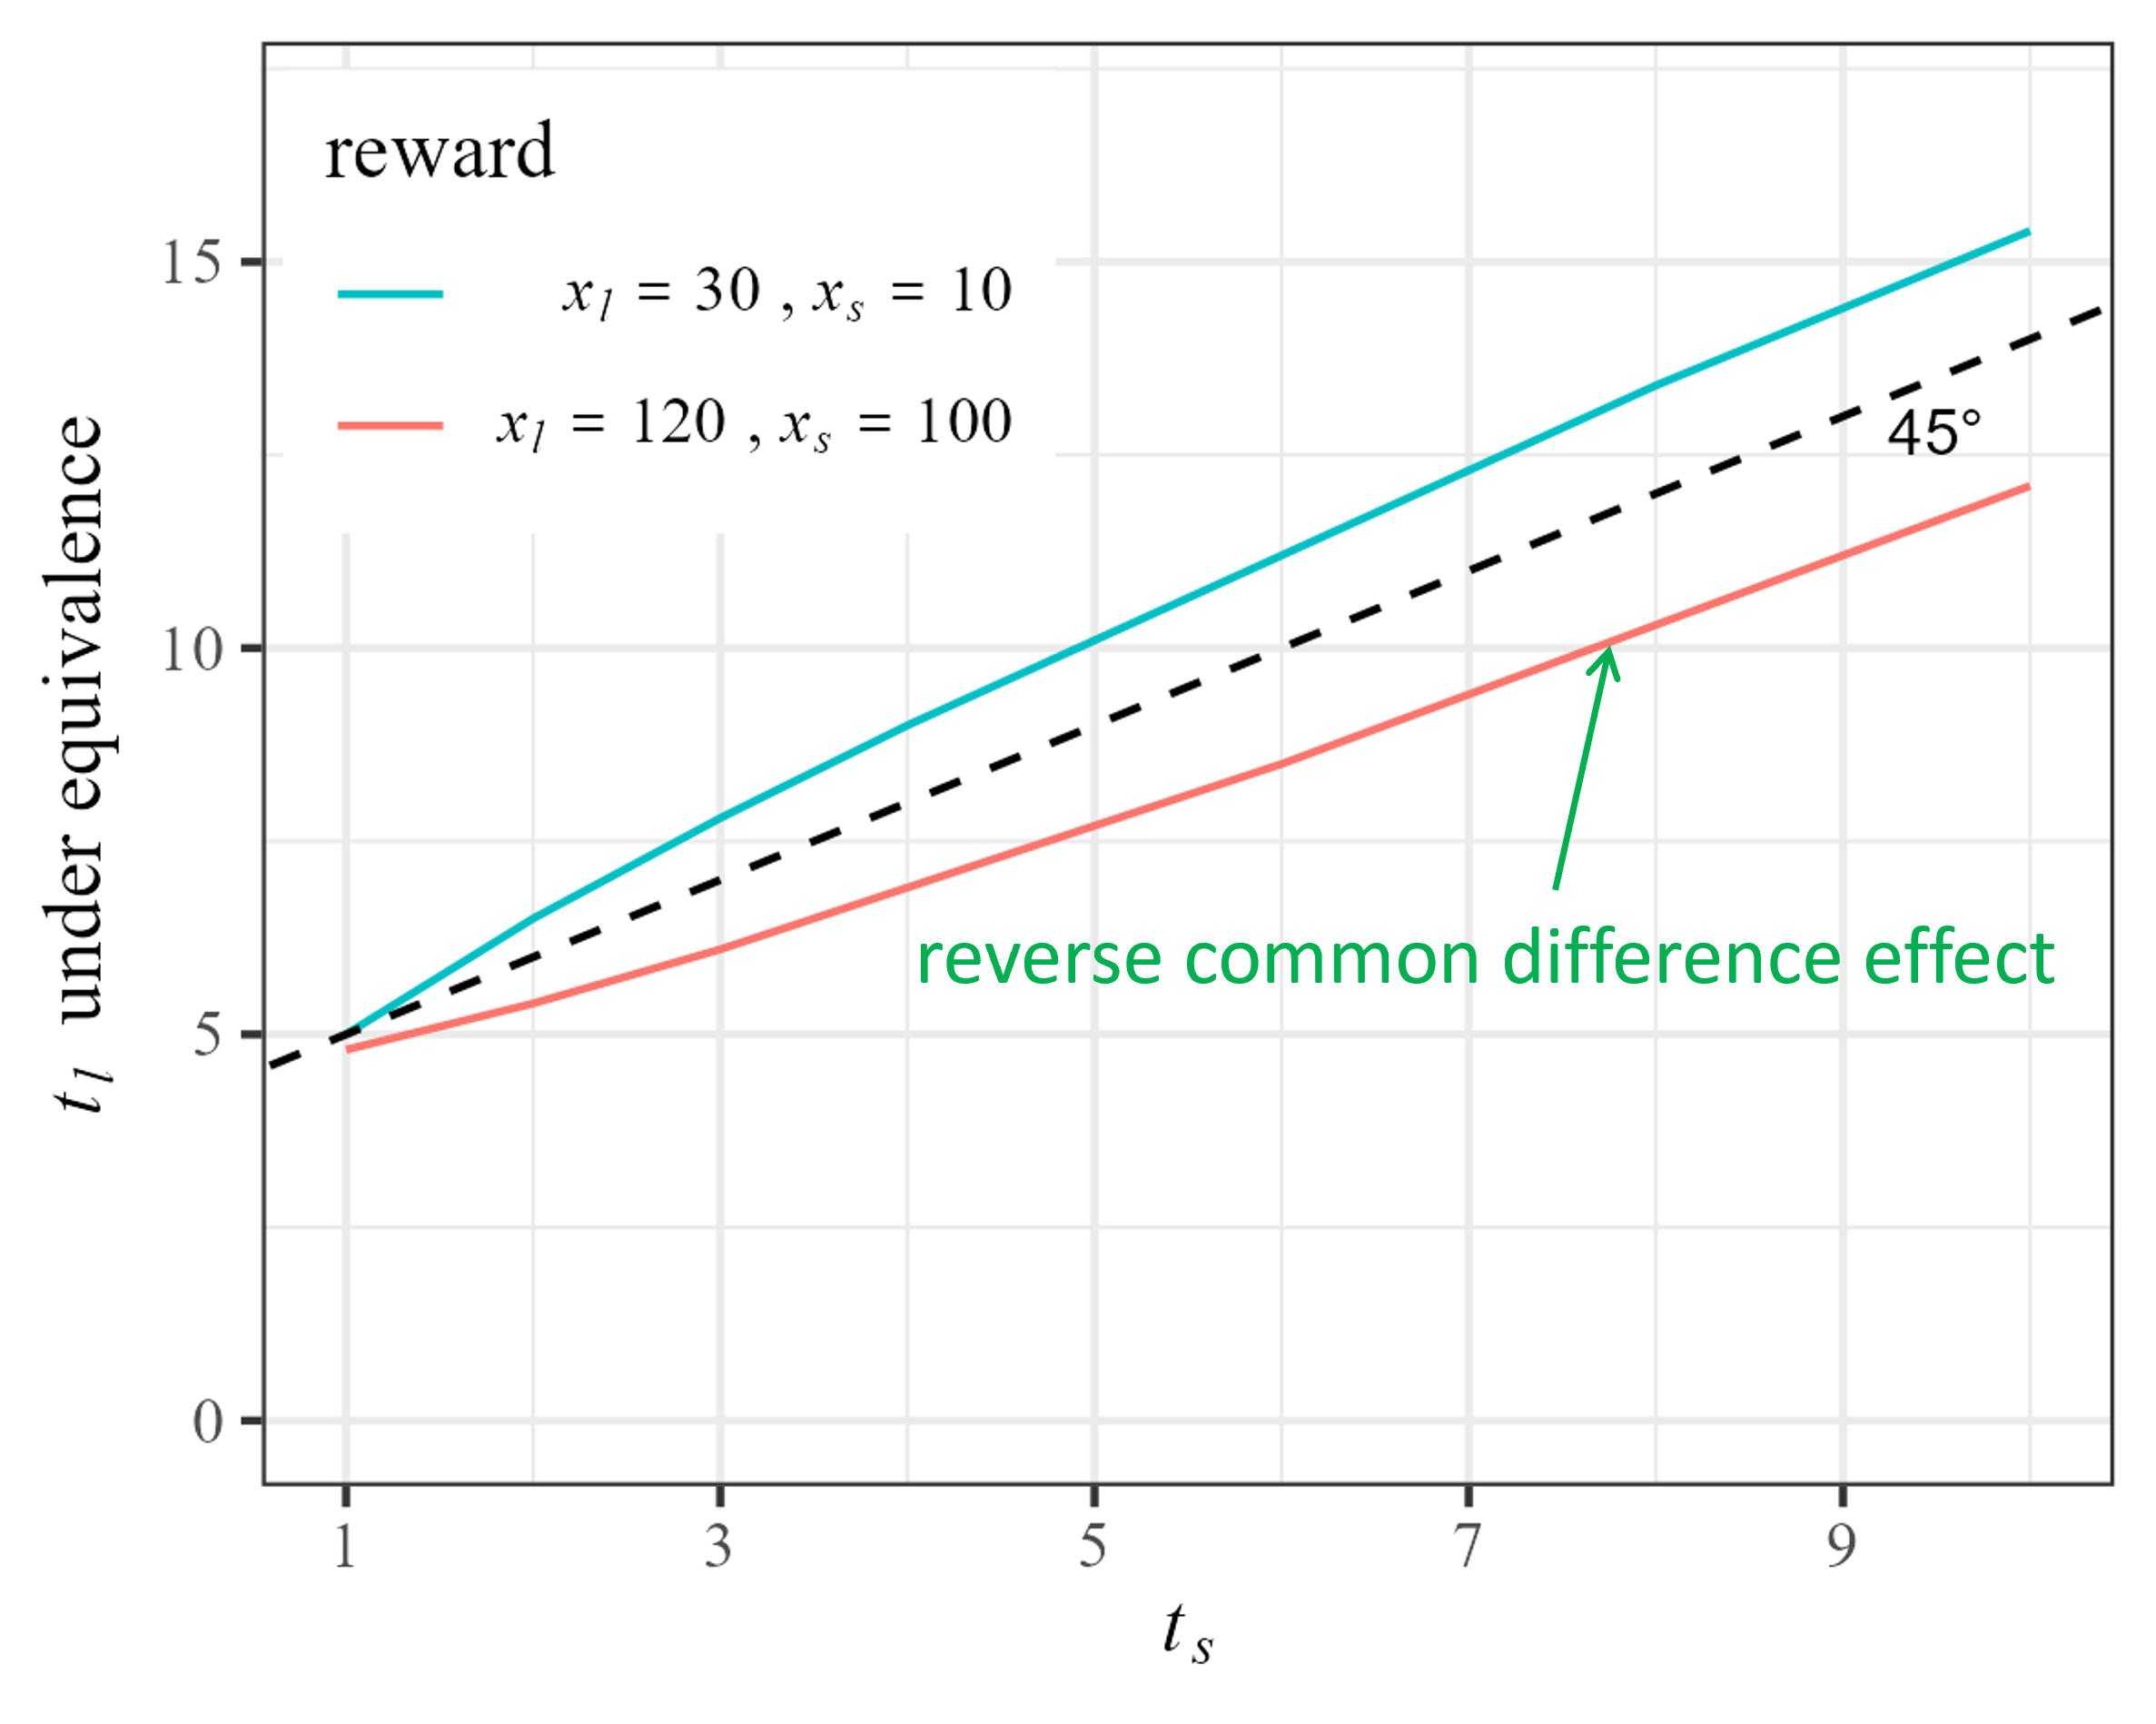
\includegraphics[width=0.65\textwidth]{figures/common_diff.png}   
  \caption{The common difference effect and its reverse}
  \vspace{8pt}
  \begin{minipage}{1.0\textwidth}
{\par\footnotesize Note: $x_l$ and $x_s$ are the positive reward levels for LL and SS. The values of LL and SS are calculated based on Equation (3). $d_t=0.75^t$, $u(x)=x^{0.6}$, $\lambda=2$. For each certain $t_s$, we identify the delay $t_l$ that makes the value of LL equivalent to SS. If the common different effect is valid, for one unit increase in $t_s$, the resultant $t_l$ should increase by a level smaller than one unit. }
\end{minipage}
  \label{fig:common_diff} 
\end{figure}

When the DM is impatient, adding a common delay would naturally make
\(v_l\) and \(v_s\) more discounted, i.e.~less attention is paid to the
corresponding rewards. Since the sum of decision weights is fixed, this
implies the the DM frees up some attention and she needs to reallocate
it across the periods in each reward sequence (LL and SS). There are
three mechanisms jointly determining whether we could observe the common
difference effect or not.

First, the existing periods with no reward delivered would grab some
attention. That is, the DM would attend more to the rewards of zero
utility, delivered in duration \([0,t_l)\) for LL and in duration
\([0,t_s]\) for SS. Given \(t_l >t_s\), the relevant duration in LL may
naturally capture more attention than that in SS. In other words, the
common delay makes the DM focus more on the waiting time in LL than in
SS, which decreases her preference for LL.

Second, the newly added time intervals also grab some attention. That
is, the DM needs to pay some attention to rewards (of zero utility as
well) delivered in duration \((t_l,t_l+\Delta t]\) in LL and in duration
\((t_s, t_s+\Delta t]\) in SS. For LL, there are already plenty of
periods over which DM has to split her attention. So, the duration
\((t_l,t_l+\Delta t]\) in LL can capture less attention than its
counterpart in SS. This increases the DM's preference for LL.

Third, the only positive reward, delivered in \(t_l\) for LL and in
\(t_s\) for SS, may draw some attention back. Given that the DM in
general tends to pay more attention to larger rewards, the positive
reward in LL can capture more ``free'' attention than that that in SS.
This also increases the preference for LL. If the latter two mechanisms
override the first mechanism, we would observe a common difference
effect in DM's choices.

\hypertarget{concavity-of-discount-function}{%
\subsection{Concavity of Discount
Function}\label{concavity-of-discount-function}}

Many time discounting models, such as exponential and hyperbolic
discounting, assume the discount function is convex in time delay. This
style of discount function predicts DM is \emph{risk seeking over time
lotteries}. To illustrate, suppose a reward of level \(x\) is delivered
at period \(t_l\) with probability \(\pi\) and is delivered at period
\(t_s\) with probability \(1-\pi\), where \(0<\pi<1\). Meanwhile,
another reward of the same level is delivered at period \(t_m\), where
\(t_m=\pi t_l +(1-\pi) t_s\). Under such discount functions, the DM
should prefer the former reward to the latter reward. For instance, she
may prefer receiving an amount of money today or in 20 weeks with equal
chance, rather than receiving it in 10 weeks with certainty. However,
experimental studies suggest that people are often \emph{risk averse
over time lotteries}, i.e.~they prefer the reward to be delivered at a
certain time \citep{onay2007intertemporal, dejarnette2020time}.

One way to accommodate the evidence about risk aversion over time
lotteries is to make the discount function concave in terms of delay.
Notably, \citet{onay2007intertemporal} find that people are more likely
to be risk averse over time lotteries when \(\pi\) is small, and to be
risk seeking when \(\pi\) is large. Given that when \(\pi\) gets larger,
\(t_m\) is also larger, we can conclude that the discount function may
be concave in delay for the near future but convex for the far future.
That is, the discount function is of inverse-S shape.
\citet{takeuchi2011non} also find evidence that supports this shape of
discount function.

In Proposition 3, we apply Equation (3) and show that the AAD is
compatible with this shape of discount function as long as the DM is
impatient and the reward level \(x\) is large enough.

\noindent \textbf{Proposition 3}: \emph{If} \(\delta =1\)\emph{, then
the discount function} \(w_T\) i\emph{s convex in} \(T\)\emph{. If}
\(0<\delta<1\)\emph{, there exist a reward threshold}
\(\underline{x}>0\) \emph{and a time threshold} \(\underline{T}>0\)
\emph{such that:}

\begin{enumerate}
\def\labelenumi{(\alph{enumi})}
\tightlist
\item
  \emph{when} \(x\leq \underline{x}\)\emph{, the discount function is
  convex in} \(T\);
\item
  \emph{when} \(x > \underline{x}\)\emph{, the discount function is
  convex in} \(T\) \emph{given} \(T\geq \underline{T}\)\emph{, and it is
  concave in} \(T\) \emph{given} \(0<T<\underline{T}\)\emph{.}
\end{enumerate}

The proof of Proposition 3 is in Appendix C. Figure
\ref{fig:discount_value_function}(a) demonstrates the convex discount
function (blue line) and the inverse-S shaped discount function (red
line) that could be yielded by Equation (3).

\begin{figure}[h]
    \centering
    \begin{subfigure}{0.49\textwidth}
        \centering
        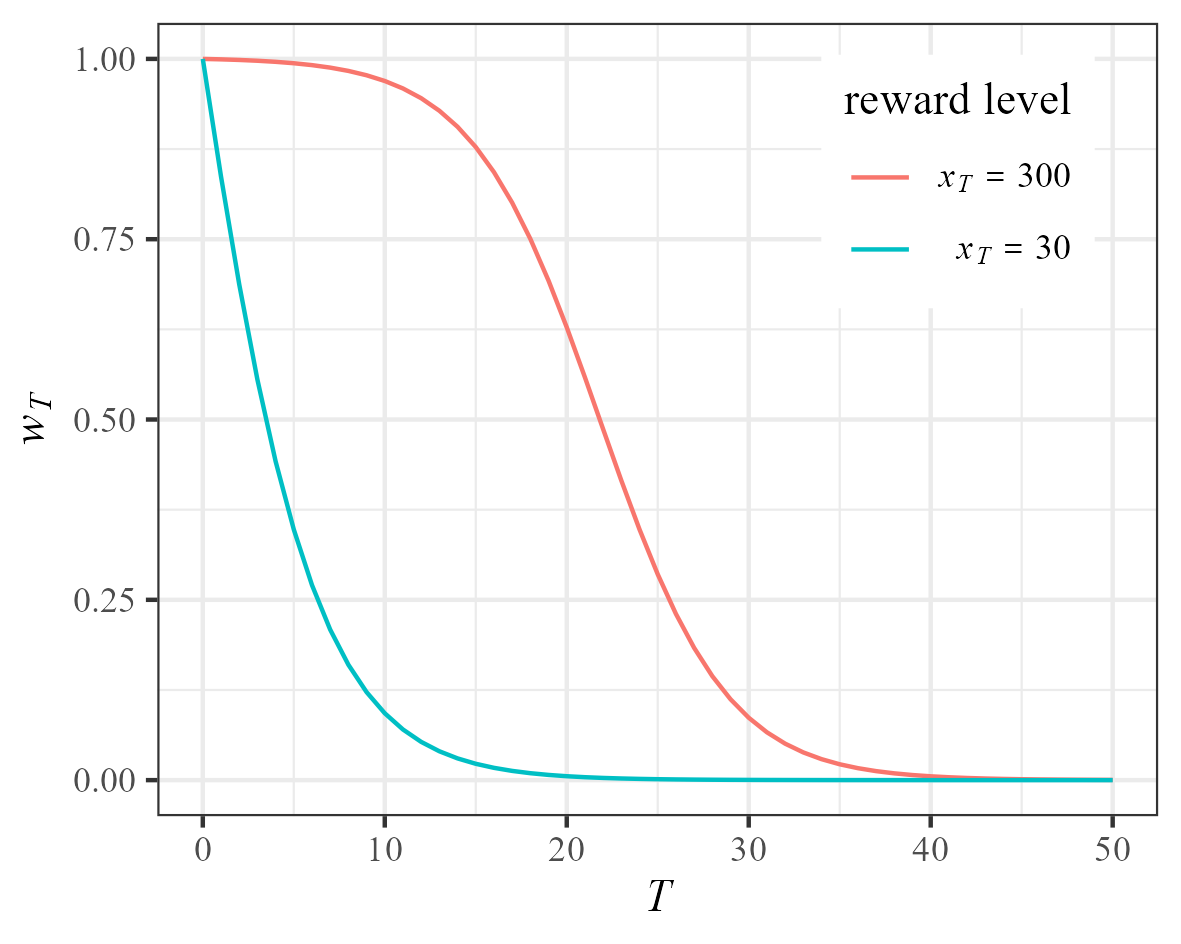
\includegraphics[width=\linewidth]{figures/concave_discount.png} 
        \caption{discount function}
    \end{subfigure}
    \hfill
    \begin{subfigure}{0.49\textwidth}
        \centering
        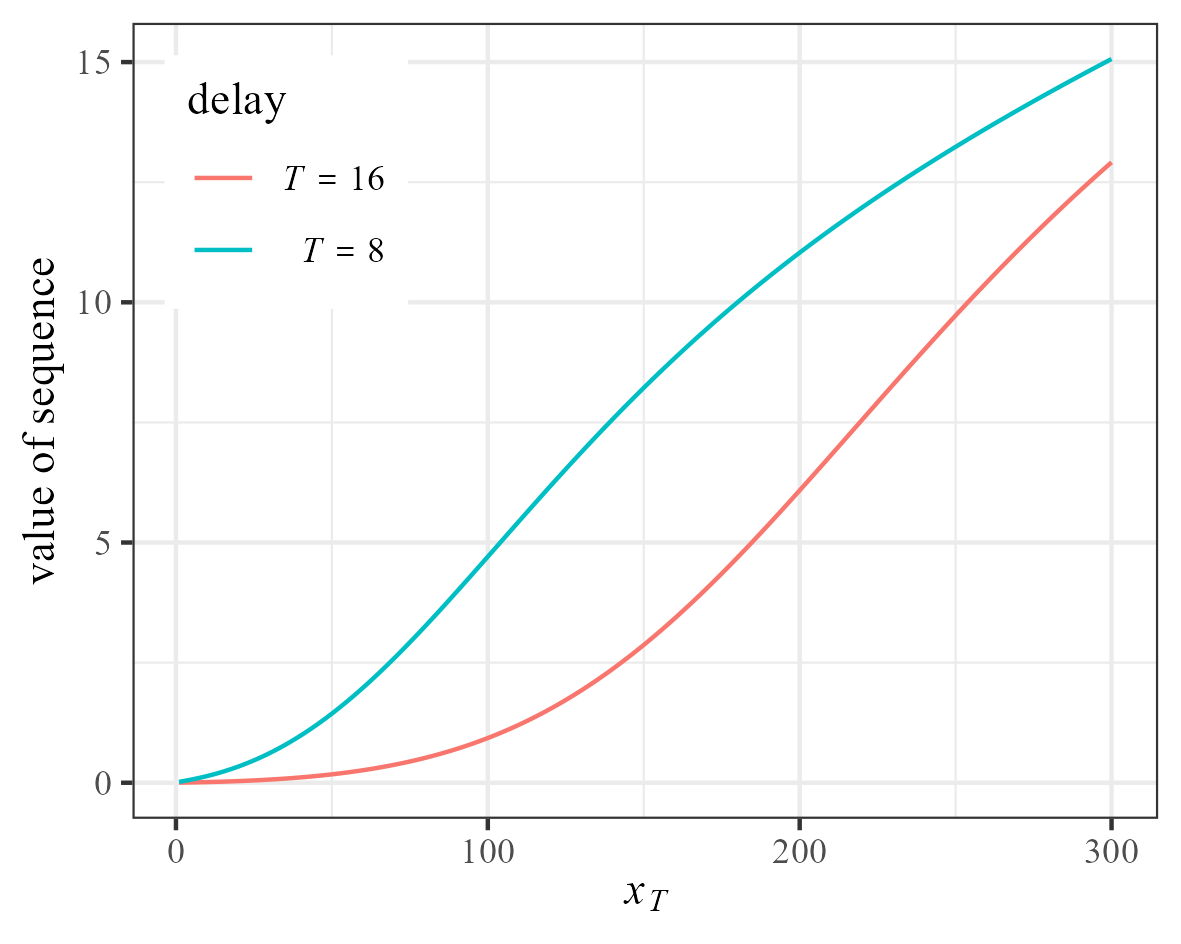
\includegraphics[width=\linewidth]{figures/s_shape_value.png}
        \caption{value function}
    \end{subfigure}
    \caption{Discount function and value function for a delayed reward}

  \vspace{8pt}
  \begin{minipage}{1.0\textwidth}
{\par\footnotesize Note: A reward of level $x_T$ is delivered at period $T$. The discount function and value function are calculated based on Equation (3). $d_t=0.75^t$, $u(x)=x^{0.6}$, $\lambda=2$.}
\end{minipage}
    
    \label{fig:discount_value_function}
\end{figure}

\hypertarget{s-shaped-value-function}{%
\subsection{S-Shaped Value Function}\label{s-shaped-value-function}}

In decision theories, it is commonly assumed that the utility function
\(u(.)\) satisfies \(u''<0\). This usually suggests the value function
of a reward is concave. However, empirical evidence suggests that the
value functions are often S-shaped. Such S-shaped value functions can be
generated by various sources, such as reference dependence
\citep{kahneman1979prospect} and efficient coding of numbers
\citep{louie2012efficient}. Through the AAD model, we provide a novel
account for S-shaped value function based on the insight that larger
rewards capture more attention.

Consider a reward of level \(x\) delivered at period \(T\). Its value
function can be represented by \(U(x,T)=w_T(x)u(x)\). We assume
\(u'>0\), \(u''<0\), and \(w_T\) is determined by Equation (3). \(w_T\)
is increasing with \(x\) as the DM tends to pay more attention to larger
rewards. Both functions \(u(x)\) and \(w_T(x)\) are concave in \(x\); so
when \(x\) is small, they both grow fast. At some conditions, it is
possible that the product of the two functions is convex in \(x\) when
\(x\) is small enough. We derive the conditions for the S-shaped value
function in Proposition 4.

\noindent \textbf{Proposition 4}: \emph{Suppose} \(T\geq1\)\emph{,}
\(\frac{d}{dx}\left(\frac{1}{v'(x)}\right)\) \emph{is continuous in}
\((0,+\infty)\)\emph{, then:}

\begin{enumerate}
\def\labelenumi{(\alph{enumi})}
\item
  \emph{There exists a threshold} \(\bar{x} \in\mathbb{R}_{\geq0}\)
  \emph{such that} \(U(x,T)\) \emph{is strictly concave in} \(x\)
  \emph{when} \(x\in [\bar{x},+\infty)\)\emph{;}
\item
  \emph{If} \(\frac{d}{dx}\left(\frac{1}{v'(x)}\right)\) \emph{is
  right-continuous at} \(x=0\) \emph{and}
  \(\frac{d}{dx}\left(\frac{1}{v'(0)}\right)<1\)\emph{, there exists a
  threshold} \(x^*\) \emph{in} \((0, \bar{x})\) \emph{such that, for
  any} \(x\in (0,x^*)\)\emph{,} \(U(x,T)\) \emph{is strictly convex in}
  \(x\).
\item
  \emph{There exists an unit cost of attention adjustment} \(\lambda^*\)
  \emph{and an interval} \((x_1,x_2)\) \emph{such that, if}
  \(\lambda<\lambda^*\)\emph{, for any} \(x\in(x_1,x_2)\)\emph{,}
  \(U(x,T)\) \emph{is strictly convex in} \(x\)\emph{, where}
  \(\lambda^*>0\) \emph{and} \((x_1,x_2)\subset(0,\bar{x})\)\emph{.}
\end{enumerate}

The proof of Proposition 4 is in Appendix D. Proposition 4 implies, if
the derivative of \(\frac{1}{v'(x)}\) converges to a small number when
\(x\rightarrow 0^+\), or the unit cost of attention adjustment
\(\lambda\) is small enough, the value function \(U(x,T)\) will be an
S-shaped in some interval of \(x\). Figure
\ref{fig:discount_value_function}(b) demonstrates examples of this
S-shaped value function.

\hypertarget{intertemporal-correlation-aversion}{%
\subsection{Intertemporal Correlation
Aversion}\label{intertemporal-correlation-aversion}}

Consider a DM facing two lotteries. For one lottery, she can receive
£100 today and £100 in 30 weeks with probability 1/2, and receive £3
today and £3 in 20 weeks with probability 1/2. For the other lottery,
she can receive £3 today and £100 in 30 weeks with probability 1/2, and
receive £100 today and £3 in 20 weeks with probability 1/2. In the
former lottery, rewards delivered at different periods are positively
correlated, whereas in the latter lottery, those rewards are negatively
correlated. The expected discounted utility theory predicts the DM is
indifferent between the two lotteries. However, reccent studies find the
evidence of \emph{intertemporal correlation aversion}
\citep{andersen2018multiattribute, rohde2023intertemporal}. That is,
people often prefer the latter lottery than the former one.\footnote{For
  theoretical analysis about intertemporal correlation aversion, please
  see \citet{epstein1983stationary}, \citet{epstein1989substitution},
  \citet{weil1990nonexpected}, \citet{bommier2005risk}, and
  \citet{bommier2017monotone}. The AAD model takes a similar form to the
  class of models defined in \citet{epstein1983stationary}. A key
  feature of such models is that the discount factor for future
  utilities is dependent on the utility achieved in the current period.}

For the above example, intertemporal correlation aversion can be
generated by the AAD model as follows. The AAD model assumes the DM
allocates decision weights within each specific reward sequence, which
implies she would aggregate values over time in each state. For
simplicity, suppose there are only two periods. In the state that the DM
receives £3 in two periods, suppose the DM allocates decision weight
\(w\) to the first period and \(1-w\) to the second period. Note in
Definition 1, when \(u(s_0)=u(s_1)=...=u(s_T)\), the decision weight
\(w_t\) for every period \(t\) within the reward sequence
\(s_{0\rightarrow T}\) will remain the same as the reference weight
\(d_t\). So, in the state that the DM receives £100 in two periods, the
allocation of decision weights is the same as \(w\) and \(1-w\). In the
state that the DM can receive £100 in the first period and £3 in the
second period, the reward of £100 can capture more attention so that its
decision weight, say \(w'\), is greater than \(w\). Similarly, in the
state that the DM receives £3 earlier and then £100, the decision weight
for the reward of £100, say \(1-w''\), is also greater than \(1-w\).
Therefore, the value of the lottery in which rewards are positively
correlated, can be represented by \(0.5\cdot u(3)+0.5\cdot u(100)\). By
contrast, for the lottery in which rewards are negatively correlated,
the value can be represented by
\(0.5(1-w'+w'')\cdot u(3)+0.5(1-w''+w')\cdot u(100)\). Given
\((1-w'')+w'>1-w+w>1\), the decision weight assigned to \(u(100)\),
which is \(0.5(1-w''+w')\), should be greater than 0.5. As a result, the
DM prefer the latter lottery than the former lottery.

In a more general setting, whether the AAD model can continuously
produce intertemporal correlation aversion is modulated by the unit cost
of attention adjustment \(\lambda\). To illustrate, we adopt the same
theoretical setting as \citet{bommier2005risk}. Let \((s_1,s_2)\) denote
the result of a lottery in which the DM can receive reward \(s_1\) in
period \(t_1\) and then reward \(s_2\) in period \(t_2\), where
\(t_2>t_1\geq 0\). There are two lotteries, \(L1\) and \(L2\). The
results of each lottery is of the same length of sequence. \(L1\)
generates \((x_s,y_s)\) and \((x_l,y_l)\) with equal chance, \(L_2\)
generates \((x_s,y_l)\) and \((x_l,y_s)\) with equal chance,
\(x_l>x_s>0\), \(y_l>y_s>0\). By Proposition 5, we show that in this
setting, we can always find a \(\lambda\) that makes the DM
intertemporal correlation averse.

\noindent \textbf{Proposition 5}: \emph{Suppose} \(U(L1), U(L2)\)
\emph{are the values of} \(L1\) \emph{and} \(L2\)\emph{. For any}
\(x_l>x_s>0\)\emph{,} \(y_l>y_s>0\)\emph{, any reference weights, and
any time length of lottery results, there exists} \emph{a threshold}
\(\lambda^{**}\) such that for any unit co\emph{st of attention
adjustment} \(\lambda>\lambda^{**}\), \emph{the DM would perform
intertemporal correlation aversion, i.e.} \(U(L1)<U(L2)\).

The proof of Proposition 5 is in Appendix E. The threshold
\(\lambda^{**}\) is jointly determined by \(x_l\), \(y_l\), \(y_s\), as
well as the reference weights for rewards delivered at \(t_1\) and
\(t_2\). Notably, when \(\lambda < \lambda^{**}\), the DM may be
intertemporal correlation seeking under some conditions.\footnote{To
  validate, one can set \(u(x_s)=5\), \(u(x_l)=10\), \(u(y_s)=1\),
  \(u(y_l)=3\). Suppose the results of each lottery contain only two
  periods, \(t_1\) and \(t_2\), and the reference weights are uniformly
  distributed, i.e.~\(d_{t_1}=d_{t_2}\). In this case, setting
  \(\lambda=1\) would generate intertemporal correlation seeking, while
  setting \(\lambda=100\) would generate intertemporal correlation
  aversion.} This suggests a potentially new mechanism for intertemporal
correlation aversion, that is, DM performs intertemporal correlation
aversion perhaps because she attends more to larger rewards while
attention adjustment is very costly.

\hypertarget{learning-and-inconsistent-planning}{%
\subsection{Learning and Inconsistent
Planning}\label{learning-and-inconsistent-planning}}

Suppose a DM has budget \(m\) (\(m>0\)) and is considering how to spend
it over different time periods. We can use a reward sequence \(x\) to
represent this decision problem, where the DM's spending in period \(t\)
is \(x_t\). In period 0, she wants to find a \(x\) such
that\[ \tag{3} \max_{x}\;\sum_{t=0}^T w_t u(x_t)\quad s.t. \;\sum_{t=0}^T x_t = m   \]

where \(w_t\) is the attention-adjusted discounting factor in period
\(t\). I assume
\(w_t=\delta^t e^{u(x_t)/\lambda}/\sum_{t=\tau}^T \delta^{\tau} e^{u(x_\tau)/\lambda}\)
and there is no risk under this setting.

\hypertarget{discussion}{%
\section{Discussion}\label{discussion}}

\hypertarget{relation-to-other-models-of-intertemporal-choice}{%
\subsection{Relation to Other Models of Intertemporal
Choice}\label{relation-to-other-models-of-intertemporal-choice}}

The theory most similar to AAD is the salience theory
\citep{bordalo2012salience, bordalo2013salience, bordalo2020memory}.

rational inattention

focus-weighted utility

bayesian updating and discounting

optimal precision

Relation with money/delay trade-off

\hypertarget{limitation}{%
\subsection{Limitation}\label{limitation}}

attention biases learning: learning rate is high for attended reward

sum of decision weights

\hypertarget{conclusion}{%
\section{Conclusion}\label{conclusion}}

\renewcommand\refname{Reference}
  \bibliography{reference.bib}

\newpage

\hypertarget{appendix}{%
\section*{Appendix}\label{appendix}}
\addcontentsline{toc}{section}{Appendix}

\hypertarget{a.-proof-of-proposition-1}{%
\subsection*{A. Proof of Proposition
1}\label{a.-proof-of-proposition-1}}
\addcontentsline{toc}{subsection}{A. Proof of Proposition 1}

We present the proof of sufficiency here. That is, if \(\succsim\) has
an optimal discounting representation and satisfies Axiom 1-4, then it
has an AAD representation.

\noindent \textbf{Lemma 1}: \emph{If Axiom 1 and 3 hold, for any}
\(s_{0\rightarrow T}\)\emph{, there exist} \(w_0, w_1, …, w_T > 0\)
\emph{such that}
\(s_{0\rightarrow T} \sim w_0 \cdot s_0 + ...+w_T\cdot s_T\)\emph{,
where} \(\sum_{t=0}^T w_t=1\)\emph{.}

\noindent \emph{Proof}: If \(T=1\), Lemma 1 is a direct application of
Axiom 3. If \(T\geq 2\), for any \(2\leq t\leq T\), there should exist
\(\alpha_t\in(0,1)\) such that
\(s_{0\rightarrow t}\sim \alpha_t\cdot s_{0\rightarrow t-1}+(1-\alpha_t)\cdot s_{t}\).
By state-independence and reduction of compound alternatives, we can
recursively apply such equivalence relations as follows:\[
\begin{aligned}
s_{0\rightarrow T} &\sim \alpha_{T-1}\cdot s_{0\rightarrow T-1} + (1-\alpha_{T-1})\cdot s_T \\
&\sim  \alpha_{T-1}\alpha_{T-2}\cdot s_{0\rightarrow T-2} + \alpha_{T-1}(1-\alpha_{T-2})\cdot s_{T-1} + (1-\alpha_{T-1})\cdot s_T \\
& \sim ...\\
& \sim w_0 \cdot s_0 + w_1\cdot s_1 +... +w_T\cdot s_T
\end{aligned}
\]where \(w_0=\prod_{t=0}^{T-1}\alpha_t\), \(w_T = 1-\alpha_{T-1}\), and
for \(0<t<T\),
\(w_t=(1-\alpha_{t-1})\prod_{\tau=t}^{T-1}\alpha_{\tau}\). It is easy to
show the sum of \(w_0,…,w_T\) is equal to 1. \emph{QED}.

Therefore, if Axiom 1 and 3 hold, for any reward sequence
\(s_{0\rightarrow T}\), we can always find a convex combination of all
its elements, such that the DM is indifferent between the reward
sequence and this convex combination. If \(s_{0\rightarrow T}\) is a
constant sequence, i.e.~all its elements are constant, then we can
directly assume \(\mathcal{W}\) is AAD-style. So henceforth, we discuss
whether AAD can apply to non-constant sequences.

By Lemma 2, we show adding a new reward to the end of
\(s_{0\rightarrow T}\) has no impact on the relative decision weights of
rewards in the original reward sequence.

\noindent \textbf{Lemma 2}: \emph{For any}
\(s_{0\rightarrow T+1}\)\emph{, if}
\(s_{0\rightarrow T}\sim \sum_{t=0}^T w_t \cdot s_t\) \emph{and}
\(s_{0\rightarrow T+1} \sim \sum_{t=0}^{T+1} w'_t\cdot s_t\)\emph{,
where} \(w_t, w'_t>0\) and \(\sum_{t=0}^Tw_t=1\)\emph{,}
\(\sum_{t=0}^{T+1}w'_t=1\)\emph{, then when Axiom 1-4 hold, we can
obtain} \(\frac{w'_0}{w_0}=\frac{w'_1}{w_1}=…=\frac{w'_T}{w_T}\)\emph{.}

\noindent \emph{Proof}: According to Axiom 3, for any
\(s_{0\rightarrow T+1}\), there exist \(\alpha,\zeta \in (0,1)\) such
that\[\tag{A1}
\begin{aligned}
s_{0 \rightarrow T}\sim\alpha\cdot s_{0 \rightarrow T-1} + (1-\alpha)\cdot s_T \\
s_{0\rightarrow T+1} \sim \zeta\cdot s_{0\rightarrow T} + (1-\zeta)\cdot s_{T+1}
\end{aligned}
\]On the other hand, we drawn on Lemma 1 and set\[\tag{A2}
s_{0\rightarrow T+1} \sim \beta_0\cdot s_{0 \rightarrow T-1} + \beta_1\cdot s_T + (1-\beta_0-\beta_1)\cdot s_{T+1}
\]where \(\beta_0, \beta_1 > 0\). According to Axiom 4,
\(1-\zeta=1-\beta_0-\beta_1\). So, \(\beta_1=\zeta-\beta_0\). This also
implies \(\zeta > \beta_0\).

According to Axiom 2, we suppose there exists a reward sequence \(s\)
such that
\(s \sim \frac{\beta_0}{\zeta}\cdot s_{0 \rightarrow T-1} + (1-\frac{\beta_0}{\zeta})\cdot s_T\).
By Equation (A2) and reduction of compound alternatives, we have
\(s_{0\rightarrow T+1}\sim \zeta \cdot s + (1-\zeta)\cdot s_{T+1}\).
Combining Equation (A2) with the second line of Equation (A1) and
applying transitivity and state-independence, we obtain
\(s_{0\rightarrow T} \sim \frac{\beta_0}{\zeta}\cdot s_{0 \rightarrow T-1} + (1-\frac{\beta_0}{\zeta})\cdot s_1\).

We aim to prove that for any \(s_{0\rightarrow T+1}\), we can obtain
\(\alpha=\frac{\beta_0}{\zeta}\). We show this by contradiction.

Given the symmetry of \(\alpha\) and \(\frac{\beta_0}{\zeta}\), we can
assume that \(\alpha > \frac{\beta_0}{\zeta}\). Consider the case that
\(s_{0 \rightarrow T-1} \succ s_T\). By state-independence, for any
\(c\in \mathbb{R}_{\geq 0}\), we have
\((\alpha - \frac{\beta_0}{\zeta})\cdot s_{0\rightarrow T-1} + (1-\alpha+\frac{\beta_0}{\zeta})\cdot c \succ (\alpha - \frac{\beta_0}{\zeta})\cdot s_T + (1-\alpha+\frac{\beta_0}{\zeta})\cdot c\).
By Axiom 2, there exists \(z\in \mathbb{R}_{\geq 0}\) such that
\((1-\alpha)\cdot s_T + \frac{\beta_0}{\zeta}\cdot s_{0\rightarrow T-1}\sim z\).
Given \(c\) is arbitrary, we can set
\((1-\alpha+\frac{\beta_0}{\zeta})\cdot c \sim z\). By reduction of
compound alternatives, we can derive that\[
(\alpha-\frac{\beta_0}{\zeta})\cdot s_{0\rightarrow T-1} +(1-\alpha)\cdot s_T + \frac{\beta_0}{\zeta}\cdot s_{0\rightarrow T-1} \succ (\alpha-\frac{\beta_0}{\zeta})\cdot s_T +(1-\alpha)\cdot s_T + \frac{\beta_0}{\zeta}\cdot s_{0\rightarrow T-1}
\]where the LHS can be rearranged to
\(\alpha\cdot s_{0\rightarrow T-1} + (1-\alpha)\cdot s_T\), and the RHS
can be rearranged to
\(\frac{\beta_0}{\zeta}\cdot s_{0 \rightarrow T-1} + (1-\frac{\beta_0}{\zeta})\cdot s_1\).
They both should be indifferent from \(s_{0\rightarrow T}\). This
results in a contradiction.

Similarly, in the case that \(s_T \succ s_{0 \rightarrow T-1}\), we can
also derive such a contradiction. Meanwhile, when
\(s_{0\rightarrow T}\sim s_T\), \(\alpha\) and \(\frac{\beta_0}{\zeta}\)
can be any number within \((0,1)\). In that case, we can directly set
\(\alpha = \frac{\beta_0}{\zeta}\).

Thus, we have \(\alpha = \frac{\beta_0}{\zeta}\) for any
\(s_{0\rightarrow T+1}\), which indicates
\(\frac{\beta_0}{\alpha}=\frac{\beta_1}{1-\alpha}=\zeta\). We can
recursively apply this equality to any sub-sequence
\(s_{0\rightarrow t}\) (\(t\leq T\)) of \(s_{0\rightarrow T+1}\), so
that the lemma will be proved. \emph{QED}.

Now we move on to prove Proposition 1. The proof contains six steps.

First, we add the constraints \(\sum_{t=0}^T w_t=1\) and \(w_t>0\) to
the optimal discounting problem for \(s_{0\rightarrow T}\) so that the
problem can accomodate Lemma 1. According to the FOC of its solution,
for all \(t=0,1,….,T\), we have\[\tag{A3}
f_t'(w_t)=u(s_t)+\theta
\]where \(\theta\) is the Lagrange multiplier. Given that \(f'_t(w_t)\)
is strictly increasing, \(w_t\) is increasing with \(u(s_t)+\theta\). We
define the solution as \(w_t =\phi_t(u(s_t)+\theta)\).

Second, we add a new reward \(s_{T+1}\) to the end of
\(s_{0\rightarrow T}\) and apply Lemma 2 as a constraint on optimal
discounting problem. Look at the optimal discounting problem for
\(s_{0\rightarrow T+1}\). For all \(t\leq T\), its FOC should take the
same form as Equation (A3). Hence, if the introduction of \(s_{T+1}\)
changes some \(w_t\) to \(w'_t\) (\(w'_t \neq w_t\), where \(w_t\) is
the solution to optimal discounting problem for \(s_{0\rightarrow T}\)),
the only way is through changing the multiplier \(\theta\). Suppose
introducing \(s_{T+1}\) changes \(\theta\) to \(\theta-\Delta \theta\),
we have \(w'_t = \phi_t(u(s_t)+\theta-\Delta \theta)\).

By Lemma 2, we know
\(\frac{w_0}{w'_0}=\frac{w_1}{w'_1}=…=\frac{w_T}{w'_T}\). In other
words, for \(t=0,1,…,T\), we have
\(w_t \propto \phi_t(u(s_t)+\theta-\Delta \theta)\). We can rewrite
\(w_t\) as \[\tag{A4}
w_t = \frac{\phi_t(u(s_t)+\theta-\Delta \theta)}{\sum_{\tau=0}^{T}\phi_\tau(u(s_\tau)+\theta-\Delta \theta)}
\]

Third, we show that in \(s_{0\rightarrow T}\), if we change each \(s_t\)
to \(z_t\) such that \(u(z_t)=u(s_t)+\Delta u\), the decision weights
\(w_0,…,w_T\) will remain the same. Note
\(\sum_{t=0}^T \phi_t(u(s_t)+\theta)=1\). It is clear that
\(\sum_{t=0}^T \phi_t(u(z_t)+\theta-\Delta u)=1\). Suppose changing
every \(s_t\) to \(z_t\) moves \(\theta\) to \(\theta'\) and
\(\theta'<\theta-\Delta u\). Then, we must have
\(\phi_t(u(z_t)+\theta')<\phi_t(u(z_t)+\theta-\Delta u)\) since
\(\phi_t(.)\) is strictly increasing. Summing all such decision weights
up will result in \(\sum_{t=0}^T \phi_t(u(z_t)+\theta')<1\), which
contradicts with the constraint that the sum of decision weights is 1.
The same contradiction can apply to the case that
\(\theta'>\theta-\Delta u\). Therefore, changing every \(s_t\) to
\(z_t\) must move \(\theta\) to \(\theta - \Delta u\), and each \(w_t\)
can only be moved to \(\phi_t(u(z_t)+\theta -\Delta u)\), which is
exactly the same as the original decision weight.

A natural corollary of this step is that, subtracting or adding a common
number to all intantaneous utilities within a reward sequence has no
effect on decision weights. What actually matters for determining the
decision weights is the difference between these instantaneous
utilities. This indicates, for convenience, we can subtract or add an
arbitrary number to the utility function.

In other words, for a given \(s_{0\rightarrow T}\) and \(s_{T+1}\), we
can define a new utility function \(v(.)\) such that
\(v(s_t) = u(s_t) +\theta-\Delta \theta\). So, Equation (A4) can be
rewritten as\[\tag{A5}
w_t = \frac{\phi_t(v(s_t))}{\sum_{\tau=0}^{T}\phi_\tau(v(s_\tau))}
\]If \(w_t\) takes the AAD form under the utility function \(v(.)\),
i.e.~\(w_t \propto d_t e^{v(s_t)/\lambda}\), then it should also take
the AAD form under the original utility function \(u(.)\).

Fourth, we show that in Equation (A4), \(\Delta \theta\) has two
properties: (i) \(\Delta \theta\) is strictly increasing with
\(u(s_{T+1})\); (ii) suppose \(\Delta \theta = \underline{\theta}\) when
\(u(s_{T+1})=\underline{u}\) and \(\Delta\theta=\bar{\theta}\) when
\(u(s_{T+1})=\bar{u}\), where \(\underline{u}<\bar{u}\), then for any
\(l \in(\underline{\theta},\bar{\theta})\), there exists
\(u(s_{T+1})\in(\underline{u},\bar{u})\) such that
\(\Delta \theta = l\).

The property (i) can be shown by contradiction. Let
\(\{w'_t\}_{t=0}^{T+1}\) denote a sequence of decision weights for
\(s_{0\rightarrow T+1}\). Suppose \(u(s_{T+1})\) is increased but
\(\Delta \theta\) is constant. In this case, each of \(w'_0,…,w'_T\)
should also be constant. However, \(w'_{T+1}\) should increase as it is
strictly increasing with \(u(s_{T+1})+\theta-\Delta \theta\) (as
\(\theta\) is determined only by the optimal discounting problem for
\(s_{0\rightarrow T}\), any operations on \(s_{T+1}\) should have no
effect on \(\theta\)). This contradicts with the constraint that
\(\sum_{t=0}^{T+1} w'_t =1\). The only way to avoid such contradictions
is to set \(\Delta \theta\) strictly increasing with \(s_{T+1}\), so
that \(w'_0,…,w'_T\) are decreasing with \(u(s_{T+1})\).

For property (ii), note that given \(s_{0\rightarrow T+1}\) and
\(\theta\), \(\Delta\theta\) is defined as the solution to
\(\sum_{t=0}^{T+1} \phi_t(u(s_t)+\theta-\Delta\theta)=1\). For any
arbitrary number \(l\in(\underline{\theta},\bar{\theta})\), the proof of
property (ii) consists of two stages. First, for period \(t=0,1,…,T\),
we need to show \(u(s_t)+\theta-l\) is in the domain of \(\phi_t(.)\).
Second, for period \(T+1\), we need to show given any
\(\omega\in(0,1)\), there exists \(u(s_{T+1})\in \mathbb{R}\) such that
\(\phi_{T+1}(u(s_{T+1})+\theta-l)=\omega\).

For the first stage, note \(\phi_t(.)\) is the inverse function of
\(f'_t(.)\). Suppose when \(\Delta\theta=\bar{\theta}\), we have
\(f'_t(w^{a}_t)=u(s_t)+\theta-\bar{\theta}\), and when
\(\Delta\theta=\underline{\theta}\), we have
\(f'_t(w^{b}_t)=u(s_t)+\theta-\underline{\theta}\). For any
\(l\in(\underline{\theta},\bar{\theta})\), we have
\(u(s_t)+\theta-l \in (f'_t(w^a_t),f'_t(w^b_t))\). Given that
\(f'_t(.)\) is continuous and strictly increasing, there must be
\(w_t\in(w^a_t,w^b_t)\) such that \(f'_t(w_t)=u(s_t)+\theta-l\). So,
\(u(s_t)+\theta-l\) is in the domain of \(\theta_t(.)\). For the second
stage, given an arbitrary \(\omega\in(0,1)\), we can directly set
\(u(s_{T+1})=f'(\omega)-\theta+l\), so that the target condition is
satisfied.

A corollary of this step is that we can manipulate \(\Delta \theta\) in
Equation (A4) at any level between \([\underline{\theta},\bar{\theta}]\)
by changing a hypothetical \(s_{T+1}\).

Fifth, we show \(\ln \phi_t(.)\) is linear under some condition. To do
this, let us add a hypothetical \(s_{T+1}\) to the end of \(s_T\) and
let \(w'_t=\phi_t(v(s_t))\) denote the decision weights for
\(s_{0\rightarrow T+1}\). We can change the hypothetical \(s_{T+1}\)
within the set \(\{s_{T+1}|v(s_{T+1})\in[\underline{v},\bar{v}]\}\) and
see what will happen to the decision weights from period 0 to period
\(T\). Suppose this changes each \(w'_t\) to \(\phi_t(v(s_t)-\eta)\).
Set \(\eta=\underline{\eta}\) when \(u(s_{T+1})=\underline{v}\) and
\(\eta=\bar{\eta}\) when \(u(s_{T+1})=\bar{v}\). By Equation (A5), we
have\[\tag{A6}
\frac{\phi_t(v(s_t))}{\sum_{\tau=0}^{T}\phi_\tau(v(s_\tau))} = \frac{\phi_t(v(s_t)-\eta)}{\sum_{\tau=0}^{T}\phi_\tau(v(s_\tau)-\eta)}
\]For each \(t=0,1,...,T\), we can rewrite \(\phi_t(v(s_t))\) as
\(e^{\ln \phi_t(v(s_t))}\). For the LHS of Equation (A6), multiplying
both the numerator and the denominator by a same number will not affect
the value. Therefore, Equation (A6) can be rewritten as \[
\frac{e^{\ln\phi_t(v(s_t))-\kappa\eta}}{\sum_{\tau=0}^{T}e^{\ln\phi_\tau(v(s_\tau))-\kappa\eta}} = \frac{e^{\ln\phi_t(v(s_t)-\eta)}}{\sum_{\tau=0}^{T}e^{\ln\phi_\tau(v(s_\tau)-\eta)}}
\]where \(\kappa\) can be any constant number. By properly selecting
\(\kappa\), for all \(t=0,1,...,T\), we can obtain\[\tag{A7}
\ln \phi_t(v(s_t))-\kappa\eta=\ln \phi_t(v(s_t)-\eta)
\]as long as \(\eta \in [\underline{\eta},\bar{\eta}]\). Since
\(\ln\phi_t(.)\) is strictly increasing, for any \(\eta\neq 0\), we have
\(\kappa>0\).

Finally, we denote the maximum and minimum of \(\{v(s_t)\}_{t=0}^T\) by
\(v_{\max}\) and \(v_{\min}\), and show that Equation (A7) can hold if
\(\eta = v_{\max} - v_{\min}\). That implies
\(v_{\max}-v_{\min}\in [\underline{\eta},\bar{\eta}]\), where
\(\underline{\eta}, \bar{\eta}\) are the realizations of \(\eta\) at the
points of \(v(s_{T+1})=\underline{v}\) and \(v(s_{T+1})=\bar{v}\).
Obviously, \(\underline{\eta}\) can take the value
\(\underline{\eta}=0\). Thus, we focus on whether \(\bar{\eta}\) can
take a value \(\bar{\eta}\geq v_{\max}-v_{\min}\).

The proof is similar with the fourth step and consists of two stages.
First, for \(t=0,1,…,T\), we show \(v(s_t)-v_{\max}+v_{\min}\) is in the
domain of \(\phi_t(.)\). That is, under some \(w_t\), we have
\(f'_t(w_t)=v(s_t)-v_{\max}+v_{\min}\). Note in a non-constant reward
sequence, \(v_{\max}-v_{\min}\in(0,+\infty)\). On the one hand, Equation
(A5) indicates that the equation \(f'_t(\omega)=v(s_t)\) has a solution
\(\omega\). On the other hand, by Definition 2, we know
\(\lim_{w_t\rightarrow 0}f'_t(w_t)=-\infty\). Given \(f'_t(w_t)\) is
continuous and strictly increasing, there must be a solution \(w_t\)
lying in \((0,\omega)\) for equation
\(f'_t(w_t)=v(s_t)-v_{\max}+v_{\min}\). Second, we show that for any
\(\omega'\in(0,1)\), there exists some \(v(s_{T+1})\) such that
\(\phi_{T+1}(v(s_{T+1})-v_{\max}+v_{\min})=\omega'\). This can be
achieved by setting \(v(s_{T+1})=f'_{T+1}(\omega')+v_{\max}-v_{\min}\).

As a result, for any period \(t\) in \(s_{0\rightarrow T}\), by Equation
(A7), we have \(\ln \phi_t(v(s_t))=\ln\phi_t(v(s_t)-\eta)+\kappa\eta\)
so long as \(\eta\in[0,v_{\max}-v_{\min}]\), where \(\kappa>0\). We can
rewrite each \(\ln \phi_t(v(s_t))\) as
\(\ln \phi_t(v_{\min})+\kappa[v(s_t)-v_{\min}]\). Therefore, we
have\[\tag{A8}
w_t \propto \phi_t(v_{\min})\cdot e^{\kappa[v(s_t)-v_{\min}]}
\]and \(\sum_{t=0}^T w_t=1\). In Equation (A8), setting
\(\phi_t(v_{\min})=d_t\), \(\lambda = 1/\kappa\), and apply the
corollary of the third step, we can conclude that
\(w_t\propto d_t e^{u(s_t)/\lambda}\), which is of the AAD form.

\hypertarget{b.-proof-of-proposition-2}{%
\subsection*{B. Proof of Proposition
2}\label{b.-proof-of-proposition-2}}
\addcontentsline{toc}{subsection}{B. Proof of Proposition 2}

Note the instantaneous utilities of LL and SS are \(v_l\) and \(v_s\),
and the delays for LL and SS are \(t_l\) and \(t_s\). According to
Equation (3), the common difference effect implies that, if\[ \tag{B1}
\frac{v_s}{1+G(t_s)e^{-v_s}} = \frac{v_l}{1+G(t_l)e^{-v_l}}
\]then for any \(\Delta t \geq 0\), we have \[ \tag{B2}
\frac{v_s}{1+G(t_s+\Delta t)e^{-v_s}} < \frac{v_l}{1+G(t_l+\Delta t)e^{-v_l}}
\]If \(G(T)=T\), we have \(G(t+\Delta t) = G(t) + \Delta t\). In this
case, combining Equation (B1) and (B2), we can obtain\[ \tag{B3}
\frac{\Delta t e^{-v_s}}{v_s} > \frac{\Delta t e^{-v_l}}{v_l}
\]Given that function \(\psi(v) = e^{-v}/v\) is decreasing with \(v\) so
long as \(v>0\), Equation (B3) is valid.

If \(G(T) = \frac{1}{1-\delta}(\delta^{-T}-1)\), we have\[
1+G(t+\Delta t)e^{-v} = \delta^{-\Delta t}[1+G(t)e^{-v}]+(\delta^{-\Delta t}-1)(\frac{e^{-v}}{1-\delta}-1)
\] Thus, combining Equation (B1) and (B2), we can obtain\[\tag{B4}
(\delta^{-\Delta t}-1)\frac{\frac{e^{-v_s}}{1-\delta}-1}{v_s} >
(\delta^{-\Delta t}-1)\frac{\frac{e^{-v_l}}{1-\delta}-1}{v_l}
\] Given that \(0<\delta<1\), we have \(\delta^{-\Delta t}>1\). So,
Equation (B4) is valid if and only if\[\tag{B5}
\frac{1}{v_s}-\frac{1}{v_l}<\frac{1}{1-\delta}(\frac{e^{-v_s}}{v_s}-\frac{e^{-v_l}}{v_l})
\] By Equation (B1), we know that\[\tag{B6}
\frac{1}{v_s}-\frac{1}{v_l}=\frac{1}{1-\delta}\left[\frac{(\delta^{-t_l}-1)e^{-v_l}}{v_l} -\frac{(\delta^{-t_s}-1)e^{-v_s}}{v_s}\right]
\] Combining Equation (B5) and (B6), we have\[
\delta^{-t_l}\frac{e^{-v_l}}{v_l}<\delta^{-t_s}\frac{e^{-v_s}}{v_s} \Longleftrightarrow v_l - v_s + \ln \left(\frac{v_l}{v_s}\right)>-(t_l-t_s)\ln\delta
\]

\hypertarget{c.-proof-of-proposition-3}{%
\subsection*{C. Proof of Proposition
3}\label{c.-proof-of-proposition-3}}
\addcontentsline{toc}{subsection}{C. Proof of Proposition 3}

Suppose a positve reward \(x\) is delivered at period \(T\). By Equation
(3), if \(w_T\) is convex in \(T\), we should have
\(\frac{\partial^2 w_T}{\partial T^2}\geq 0\). This
implies\[\tag{C1} 2G'(T)^2\geq(G(T)+e^{v(x)})G''(T) \]

If \(\delta=1\), then \(G(T)=T\). We have \(G'(T)=1\), \(G''(T)=0\).
Thus, Equation (C1) is always valid.

If \(0<\delta<1\), then \(G(T)=(1-\delta)^{-1}(\delta^{-T}-1)\). We have
\(G'(T)=(1-\delta)^{-1}(-\ln\delta)\delta^{-T}\),
\(G''(t)=(-\ln\delta)G'(T)\). Thus, Equation (C1) is valid when
\[\tag{C2} \delta^{-T}\geq(1-\delta)e^{v(x)}-1 \]Given \(T>0\), Equation
(C2) holds true in two cases. The first case is
\(1\geq (1-\delta)e^{v(x)}-1\), which implies that \(v(x)\) is no
greater than a certain threshold \(v(\underline{x})\), where
\(v(\underline{x})=\ln(\frac{2}{1-\delta})\). The second case is that
\(v(x)\) is above \(v(\underline{x})\) and \(T\) is above a threshold
\(\underline{t}\). In the second case, we can take the logarithm on both
sides of Equation (C2). It yields
\(\underline{t}=\frac{\ln[(1-\delta)\exp\{v(x)\}-1]}{\ln(1/\delta)}\).

\hypertarget{d.-proof-of-proposition-4}{%
\subsection*{D. Proof of Proposition
4}\label{d.-proof-of-proposition-4}}
\addcontentsline{toc}{subsection}{D. Proof of Proposition 4}

For convenience, we use \(v\) to represent \(v(x)\equiv u(x)/\lambda\),
and use \(U\) to represent \(U(x,T)\). Set \(g= G(T)\). The first-order
derivative of \(U\) with respect to \(x\) can be written as\[\tag{D1}
\frac{\partial U}{\partial x}=v'\frac{e^v+U}{e^v+g}
\]If \(U\) is strictly concave in \(x\), we should have
\(\frac{\partial^2 U}{\partial x^2}<0\). By Equation (D1), we calculate
the second-order derivative of \(U\) with respect to \(x\), and
rearrange this second-order condition to\[\tag{D2}
2\zeta(v)+\frac{1}{1+v\zeta(v)}-1<\frac{-v''}{(v')^2}\equiv\frac{d}{dx}\left(\frac{1}{v'}\right)
\]

where \(\zeta(v)=g/(g+e^v)\). Since \(v''<0\), the RHS of Equation (D2)
is clearly positive.

To prove the first part of Proposition 4, we can show that when \(x\) is
large enough, the LHS of Equation (D2) will be non-positive. To make the
LHS non-positive, we require\[\tag{D3}
\zeta(v)+\frac{1}{v}\leq\frac{1}{2}
\]hold true. Note that \(\zeta(v)\) is decreasing in \(v\), and \(v\) is
increasing in \(x\). Hence, \(\zeta(v)+\frac{1}{v}\) is decreasing in
\(x\). Besides, it approaches \(+\infty\) when \(x\rightarrow0\) and
approaches 0 when \(x\rightarrow +\infty\). When
\(\frac{d}{dx}\left(\frac{1}{v'(x)}\right)\) is continuous, there must
be a unique realization of \(x\) in \((0,+\infty)\), say \(\bar{x}\),
making the equality in Equation (D3) valid. Moreover, when
\(x\geq\bar{x}\), Equation (D3) is always valid. In such cases,
\(U(x,T)\) is concave in \(x\).

To prove the second part, first note that when \(x=0\), the LHS of
Equation (D2) will become \(\frac{2g}{g+1}\). If
\(\frac{d}{dx}\left(\frac{1}{v'(0)}\right)\) is smaller than this
number, then the LHS of Equation (D2) should be greater than the RHS at
the point of \(x=0\). Meanwhile, from the first part of the current
proposition, we know the LHS is smaller than the RHS at the point of
\(x=\bar{x}\). Thus, given \(\frac{d}{dx}\left(\frac{1}{v'(x)}\right)\)
is continuous in \([0,\bar{x}]\), there must also be a point within
\([0,\bar{x}]\), such that the LHS equals the RHS. Let \(x^*\) denote
the minimum of \(x\) that makes the equality valid. Then, for any
\(x\in(0,x^*)\), we must have that the LHS of Equation (D2) is greater
than the RHS, which implies \(U(x,T)\) is convex in \(x\). Given that
\(T\geq1\), we have \(g\geq1\) and thus \(\frac{2g}{g+1}\geq 1\).
Therefore, when \(\frac{d}{dx}\left(\frac{1}{v'(0)}\right)<1\),
\(U(x,t)\) can be convex in \(x\) for any \(x\in(0,x^{*})\), regardless
of \(g\).

The prove the third part, note \(v(x)=u(x)/\lambda\). So, \[
\frac{d}{dx}\left(\frac{1}{v'}\right)=\lambda\frac{d}{dx}\left(\frac{1}{u'}\right)
\]We arbitrarily draw a point from \((0,\bar{x})\) and derive the range
\(\lambda\) relative to this point. For simplicity, we choose
\(x=\ln g\). In this case, the LHS of Equation (D2) becomes
\(\frac{2}{2+\ln g}\). Define a function \(\xi(x)\), where \(\xi\) is
the value of the LHS of Equation (D2) minus its RHS. Note \(\xi(x)\) is
continuous at \(x=\ln g\). Therefore, for any positive real number
\(b\), there must exist a positive real number \(c\) such that, when
\(x\in(\ln g-c,\ln g+c)\), we have\[\tag{D4}
\xi(\ln g)-b<\xi(x)<\xi(\ln g)+b
\]If \(\xi(\ln g)-b\geq 0\), then \(\xi(x)\) will keep positive for all
\(x\in(\ln g-c,\ln g+c)\), which implies the LHS of Equation (D2) is
always greater than its RHS.

Now we derive the condition for \(\xi(\ln g)-b\geq 0\). Suppose when
\(x=\ln g\), \(\frac{d}{dx}\left(\frac{1}{u'}\right)=a\) (note at this
point we have \(\frac{d}{dx}\left(\frac{1}{u'}\right)<+\infty\)).
Combining with Equation (D3), we know that
\(\xi(\ln g)-b =\frac{2}{2+\ln g}-\lambda a-b\). Letting this value be
non-negative, we obtain\[\tag{D5}
\lambda \leq \frac{2}{a(2+\ln g)}-\frac{b}{a}
\]Given that \(T\geq1\), we have \(g\geq 1\) and thus
\(\frac{2}{2+\ln g}\) should be positive. Meanwhile, given that \(u'>0\)
and \(u''<0\), \(a\) should also be positive. Since \(b\) can be any
positive number, Equation (D5) holds if
\(\lambda <\frac{2}{a(2+\ln g)}\). That is, when \(\lambda\) is positive
but smaller than a certain threshold, there must be an interval
\((\ln g-c,\ln g+c)\) such that the LHS of Equation (D2) is greater than
the RHS. Set \(x_1 = \max\{0,\ln g-c\}\),
\(x_2=\min\{\bar{x}, \ln g +c\}\). When \(x\in (x_1,x_2)\), function
\(U(x,T)\) must be convex in \(x\).

\hypertarget{e.-proof-of-proposition-5}{%
\subsection*{E. Proof of Proposition
5}\label{e.-proof-of-proposition-5}}
\addcontentsline{toc}{subsection}{E. Proof of Proposition 5}

The proof consists of four steps. First, we write the expressions for
\(U(L1)\) and \(U(L2)\). Suppose the time length of each lottery result
is \(T\). For a period \(\tau\) at which no reward is delivered, the
instantaneous utility is zero. Let \(\Omega\) denote the set of all such
period \(\tau\), then
\(\Omega=\{\tau\,|\,0\leq\tau\leq T,\;\tau \neq t_1,t_2\}\). For any
\(j,k\in\{s,l\}\), we define \(\phi_j=d_{t_1}e^{v(x_j)}\) and
\(\eta_k=d_{t_2}e^{v(y_k)}\), where \(v(s)=u(s)/\lambda\), and \(d_t\)
represents the reference weight for any reward delivered at period
\(t\).

For a given lottery result \((s_1,s_2)\), we denote the decision weight
of each positive reward by \(w_{t_1}\) and \(w_{t_2}\). By the
definition of AAD, we have\[
w_{t_1} = \frac{\phi_j}{\phi_j + \eta_k +D} \quad ,\quad
w_{t_2} = \frac{\eta_k}{\phi_j + \eta_k +D}
\]where \(j,k\in\{s,l\}\), \(D=\sum_{\tau\in\Omega} d_{\tau}\geq 0\).
The value of a lottery \(L\) can be written as
\(U(L)=w_{t_1}u(s_1)+w_{t_2}u(s_2)\). Hence, \[\tag{E1}
\begin{aligned}
U(L1)=0.5\frac{\phi_s u(x_s)+\eta_s u(y_s)}{\phi_s+\eta_s+D} + 0.5\frac{\phi_l u(x_l)+\eta_l u(y_l)}{\phi_l+\eta_l+D} \\
U(L2)=0.5\frac{\phi_s u(x_s)+\eta_l u(y_l)}{\phi_s+\eta_l+D} + 0.5\frac{\phi_l u(x_l)+\eta_s u(y_s)}{\phi_l+\eta_s+D}
\end{aligned}
\]We observe that, when \(x_l=x_s\), we have \(U(L1)=U(L2)\).

Second, suppose we increase \(x_l\) from \(x_s\) by an increment. This
increases both \(U(L1)\) and \(U(L2)\) (either by a positive or a
negative number). To make \(U(L1)<U(L2)\), this increment should
increase \(U(L2)\) by a greater number than \(U(L1)\). Specifically, we
assume \(U(L2)\) is increasing faster than \(U(L1)\) at any level of
\(x_l\). That is, the partial derivative of \(U(L2)\) in terms of
\(x_l\) is always greater than that of \(U(L1)\). Given \(\phi_l\) is
increasing in \(x_l\), to see this, we can take partial derivatives in
terms of \(\phi_l\).

In each line of Equation (E1), note only the second term contains
\(x_l\). Thus, we focus on the difference between the second terms. The
second term of the \(U(L1)\) is influenced by \(y_l\), while that of the
\(U(L2)\) is influenced by \(y_s\), where \(y_l>y_s\). Thus, we can
construct a function \(\xi\) such that\[
\xi(\phi_l,\eta) = \frac{\phi_l \cdot v(x_l)+\eta\cdot v(y)}{\phi_l+\eta+D}
\]where \(\eta=d_{t_2}e^{v(y)}\). In reverse, we can define
\(v(x_l)=\ln(\phi_l/d_{t_1})\) and \(v(y)=\ln(\eta/d_{t_2})\). The
function \(\xi\) is similar to the second term of each line, but note we
replace \(u(.)\) by \(v(.)\). When \(y=y_l\), \(\xi\) is proportional to
the second term of \(U(L1)\). When \(y=y_s\), \(\xi\) is proportional to
the second term of \(U(L2)\) (by the same proportion). Thus, to show
that the partial derivative of \(U(L2)\) in terms of \(x_l\) is greater
than that of \(U(L1)\), we just need to show
\(\partial \xi/\partial \phi_l\) is decreasing with \(y\) (or \(\eta\)).

Third, we take the first- and second-order partial derivatives of
\(\xi(\phi_l,\eta)\). The partial derivative of \(\xi\) in terms of
\(\phi_l\) is\[
\frac{\partial \xi}{\partial \phi_l}=\frac{(v(x_l)+1)\eta-v(y)\eta+\phi_l+D(v(x_l)+1)}{(\phi_l+\eta+D)^2}
\]We need to show that for \(y\in[y_s,y_l]\), we can obtain
\(\partial^2 \xi/\partial \phi_l\partial \eta<0\). This
implies\[\tag{E2}
(v(x_l)+v(y)+2)D-(\phi_l-\eta)(v(x_l)-v(y))+2(\phi_l+\eta)>0
\]We want Equation (E2) to hold for any \(D\geq\). Given the LHS is
increasing with \(D\), this can only be achieved when\[\tag{E3}
2(\phi_l+\eta)>(\phi_l-\eta)(v(x_l)-v(y))
\]Define \(\kappa=d_{t_2}/d_{t_1}\), \(\alpha=v(x_l)-v(y)\). Note
\(\kappa\in \mathbb{R}_{>0}\), \(\alpha\in\mathbb{R}\). Equation (E3)
can be rewritten as\[\tag{E4}
(\alpha-2)\kappa^{-1} e^{\alpha}-\alpha-2<0
\]

Fourth, based on Equation (E4), we construct a function
\(h(\alpha)=(\alpha-2)\kappa^{-1} e^\alpha-\alpha-2\). We aim to examine
whether there exists some \(\alpha\in\mathbb{R}\) that makes \(h(a)<0\).
Obviously, \(\alpha=-2\) and \(\alpha=2\) satisfy this condition.
Moreover, note \(h(\alpha)\) is decreasing in \(\alpha\) when
\((\alpha-1)e^{\alpha}\leq \kappa\) and is increasing in \(\alpha\)
otherwise. And when either \(\alpha\rightarrow -\infty\) or
\(\alpha \rightarrow +\infty\), we have
\(h(\alpha)\rightarrow +\infty\). Thus, there must be a limited interval
\((\alpha_1,\alpha_2)\) such that \(h(a)<0\) so long as
\(\alpha\in(\alpha_1,\alpha_2)\), and obviously
\([-2,2]\subset(\alpha_1,\alpha_2)\). Since \(v(s)=u(s)/\lambda\), this
implies \(\frac{u(x_l)-u(y)}{\lambda}\in(\alpha_1,\alpha_2)\).

For a given positive number \(\kappa\), the points \(\alpha_1,\alpha_2\)
are determined by the solution to
\(\frac{\alpha-2}{\alpha+2}e^{\alpha}=\kappa\). In other words, for any
\(x_l\) and \(y\in[y_s,y_l]\), we can always achieve \(U(L1)<U(L2)\) as
long as \(u(x_l)-u(y_l)\geq \lambda\alpha_1\) and
\(u(x_l)-u(y_s)\leq\lambda\alpha_2\). So, we can conclude that for any
\(x_l>x_s>0\), \(y_l>y_s>0\), any time length of lottery results and
reference weights (which determines \(D\) and \(\kappa\)), there exists
some \(\lambda\) that makes DM intertemporal correlation averse.
Specifically, all
\(\lambda>\lambda^{**} ={\max}\{\frac{u(x_l)-u(y_l)}{\alpha_1},\frac{u(x_l)-u(y_s)}{\alpha_2}\}\)
satisfy the target condition.

Notably, if \(\lambda\leq\lambda^{**}\), we have \(h(a)\geq0\), which by
Equation (E2)(E3), indicates that under some conditions such as \(D=0\),
there will be \(\partial^2 \xi/\partial \phi_l\partial \eta\geq0\) for
all \(y\in[y_s,y_l]\). In that case, at each level of \(x_l\), the
partial derivative of \(U(L1)\) in terms of \(x_l\) is greater than that
of \(U(L2)\). Or in other words, increasing \(x_l\) by an increment can
induce a greater increase in \(U(L1)\) than in \(U(L2)\), so it is
possible that \(U(L1)>U(L2)\). Therefore, DM may perform intertemporal
correlation seeking when \(\lambda\leq\lambda^{**}\).

\end{document}
